% Options for packages loaded elsewhere
\PassOptionsToPackage{unicode}{hyperref}
\PassOptionsToPackage{hyphens}{url}
%
\documentclass[
]{report}
\usepackage{lmodern}
\usepackage{amssymb,amsmath}
\usepackage{ifxetex,ifluatex}
\ifnum 0\ifxetex 1\fi\ifluatex 1\fi=0 % if pdftex
  \usepackage[T1]{fontenc}
  \usepackage[utf8]{inputenc}
  \usepackage{textcomp} % provide euro and other symbols
\else % if luatex or xetex
  \usepackage{unicode-math}
  \defaultfontfeatures{Scale=MatchLowercase}
  \defaultfontfeatures[\rmfamily]{Ligatures=TeX,Scale=1}
\fi
% Use upquote if available, for straight quotes in verbatim environments
\IfFileExists{upquote.sty}{\usepackage{upquote}}{}
\IfFileExists{microtype.sty}{% use microtype if available
  \usepackage[]{microtype}
  \UseMicrotypeSet[protrusion]{basicmath} % disable protrusion for tt fonts
}{}
\makeatletter
\@ifundefined{KOMAClassName}{% if non-KOMA class
  \IfFileExists{parskip.sty}{%
    \usepackage{parskip}
  }{% else
    \setlength{\parindent}{0pt}
    \setlength{\parskip}{6pt plus 2pt minus 1pt}}
}{% if KOMA class
  \KOMAoptions{parskip=half}}
\makeatother
\usepackage{xcolor}
\IfFileExists{xurl.sty}{\usepackage{xurl}}{} % add URL line breaks if available
\IfFileExists{bookmark.sty}{\usepackage{bookmark}}{\usepackage{hyperref}}
\hypersetup{
  pdftitle={  STAT 216 Activity Coursepack},
  hidelinks,
  pdfcreator={LaTeX via pandoc}}
\urlstyle{same} % disable monospaced font for URLs
\usepackage{color}
\usepackage{fancyvrb}
\newcommand{\VerbBar}{|}
\newcommand{\VERB}{\Verb[commandchars=\\\{\}]}
\DefineVerbatimEnvironment{Highlighting}{Verbatim}{commandchars=\\\{\}}
% Add ',fontsize=\small' for more characters per line
\usepackage{framed}
\definecolor{shadecolor}{RGB}{248,248,248}
\newenvironment{Shaded}{\begin{snugshade}}{\end{snugshade}}
\newcommand{\AlertTok}[1]{\textcolor[rgb]{0.94,0.16,0.16}{#1}}
\newcommand{\AnnotationTok}[1]{\textcolor[rgb]{0.56,0.35,0.01}{\textbf{\textit{#1}}}}
\newcommand{\AttributeTok}[1]{\textcolor[rgb]{0.77,0.63,0.00}{#1}}
\newcommand{\BaseNTok}[1]{\textcolor[rgb]{0.00,0.00,0.81}{#1}}
\newcommand{\BuiltInTok}[1]{#1}
\newcommand{\CharTok}[1]{\textcolor[rgb]{0.31,0.60,0.02}{#1}}
\newcommand{\CommentTok}[1]{\textcolor[rgb]{0.56,0.35,0.01}{\textit{#1}}}
\newcommand{\CommentVarTok}[1]{\textcolor[rgb]{0.56,0.35,0.01}{\textbf{\textit{#1}}}}
\newcommand{\ConstantTok}[1]{\textcolor[rgb]{0.00,0.00,0.00}{#1}}
\newcommand{\ControlFlowTok}[1]{\textcolor[rgb]{0.13,0.29,0.53}{\textbf{#1}}}
\newcommand{\DataTypeTok}[1]{\textcolor[rgb]{0.13,0.29,0.53}{#1}}
\newcommand{\DecValTok}[1]{\textcolor[rgb]{0.00,0.00,0.81}{#1}}
\newcommand{\DocumentationTok}[1]{\textcolor[rgb]{0.56,0.35,0.01}{\textbf{\textit{#1}}}}
\newcommand{\ErrorTok}[1]{\textcolor[rgb]{0.64,0.00,0.00}{\textbf{#1}}}
\newcommand{\ExtensionTok}[1]{#1}
\newcommand{\FloatTok}[1]{\textcolor[rgb]{0.00,0.00,0.81}{#1}}
\newcommand{\FunctionTok}[1]{\textcolor[rgb]{0.00,0.00,0.00}{#1}}
\newcommand{\ImportTok}[1]{#1}
\newcommand{\InformationTok}[1]{\textcolor[rgb]{0.56,0.35,0.01}{\textbf{\textit{#1}}}}
\newcommand{\KeywordTok}[1]{\textcolor[rgb]{0.13,0.29,0.53}{\textbf{#1}}}
\newcommand{\NormalTok}[1]{#1}
\newcommand{\OperatorTok}[1]{\textcolor[rgb]{0.81,0.36,0.00}{\textbf{#1}}}
\newcommand{\OtherTok}[1]{\textcolor[rgb]{0.56,0.35,0.01}{#1}}
\newcommand{\PreprocessorTok}[1]{\textcolor[rgb]{0.56,0.35,0.01}{\textit{#1}}}
\newcommand{\RegionMarkerTok}[1]{#1}
\newcommand{\SpecialCharTok}[1]{\textcolor[rgb]{0.00,0.00,0.00}{#1}}
\newcommand{\SpecialStringTok}[1]{\textcolor[rgb]{0.31,0.60,0.02}{#1}}
\newcommand{\StringTok}[1]{\textcolor[rgb]{0.31,0.60,0.02}{#1}}
\newcommand{\VariableTok}[1]{\textcolor[rgb]{0.00,0.00,0.00}{#1}}
\newcommand{\VerbatimStringTok}[1]{\textcolor[rgb]{0.31,0.60,0.02}{#1}}
\newcommand{\WarningTok}[1]{\textcolor[rgb]{0.56,0.35,0.01}{\textbf{\textit{#1}}}}
\usepackage{longtable,booktabs}
% Correct order of tables after \paragraph or \subparagraph
\usepackage{etoolbox}
\makeatletter
\patchcmd\longtable{\par}{\if@noskipsec\mbox{}\fi\par}{}{}
\makeatother
% Allow footnotes in longtable head/foot
\IfFileExists{footnotehyper.sty}{\usepackage{footnotehyper}}{\usepackage{footnote}}
\makesavenoteenv{longtable}
\usepackage{graphicx}
\makeatletter
\def\maxwidth{\ifdim\Gin@nat@width>\linewidth\linewidth\else\Gin@nat@width\fi}
\def\maxheight{\ifdim\Gin@nat@height>\textheight\textheight\else\Gin@nat@height\fi}
\makeatother
% Scale images if necessary, so that they will not overflow the page
% margins by default, and it is still possible to overwrite the defaults
% using explicit options in \includegraphics[width, height, ...]{}
\setkeys{Gin}{width=\maxwidth,height=\maxheight,keepaspectratio}
% Set default figure placement to htbp
\makeatletter
\def\fps@figure{htbp}
\makeatother
\setlength{\emergencystretch}{3em} % prevent overfull lines
\providecommand{\tightlist}{%
  \setlength{\itemsep}{0pt}\setlength{\parskip}{0pt}}
\setcounter{secnumdepth}{5}
\usepackage{booktabs}
\usepackage{geometry}
\usepackage[none]{hyphenat}
\usepackage{titlesec}
\usepackage{longtable}


\pagestyle{plain}

%%%% Set margins
\setlength{\topmargin}{-1cm}
\addtolength{\evensidemargin}{-1cm}
\addtolength{\oddsidemargin}{-1cm}
\addtolength{\textheight}{3cm}
\addtolength{\textwidth}{2cm}

\renewcommand*{\chaptername}{Activity}

\titleformat{\chapter}[display]
{\bfseries\Large}
{\filleft\MakeUppercase{\chaptertitlename} \Huge\thechapter}
{3ex}
{\titlerule
\vspace{1.5ex}%
\filright}
[\vspace{1.5ex}%
\titlerule]
\titlespacing*{\chapter}{0pt}{-40pt}{20pt}
\ifluatex
  \usepackage{selnolig}  % disable illegal ligatures
\fi
\usepackage[]{natbib}
\bibliographystyle{plainnat}

\title{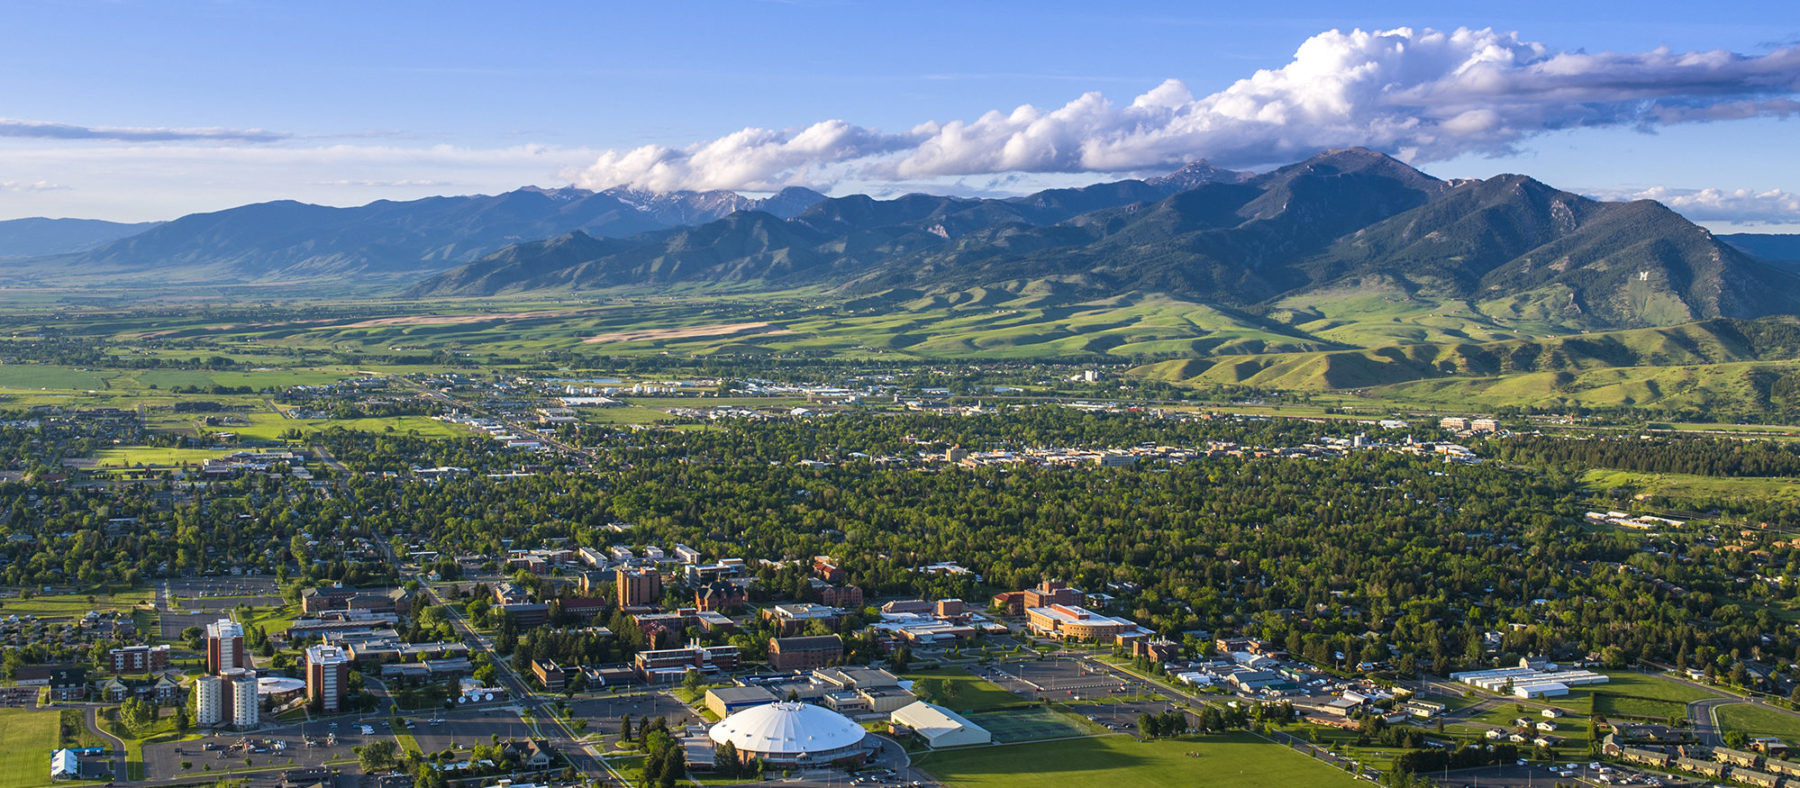
\includegraphics[width=5in,height=\textheight]{images/msu-campus.jpg}
\vspace{1cm}\\
STAT 216 Activity Coursepack}
\usepackage{etoolbox}
\makeatletter
\providecommand{\subtitle}[1]{% add subtitle to \maketitle
  \apptocmd{\@title}{\par {\large #1 \par}}{}{}
}
\makeatother
\subtitle{Fall 2020}
\author{}
\date{\vspace{-2.5em}}

\begin{document}
\maketitle

\newpage
\thispagestyle{empty}

\mbox{}

\setcounter{tocdepth}{0}
\tableofcontents

\newpage

\hypertarget{preface}{%
\chapter*{Preface}\label{preface}}
\addcontentsline{toc}{chapter}{Preface}

This coursepack accompanies the textbook for STAT 216: Introduction to Statistics at Montana State University. Each of the activities in this workbook is designed to target specific learning outcomes of the course, giving you practice with important statistical concepts in a group setting with instructor guidance. Bring this workbook with you to class each week, and take notes in the workbook as you would your own notes. A well-written complete workbook will provide an optimal study guide for exams!

\hypertarget{fall-2020-calendar-of-in-class-activities}{%
\chapter*{Fall 2020 Calendar of In-Class Activities}\label{fall-2020-calendar-of-in-class-activities}}
\addcontentsline{toc}{chapter}{Fall 2020 Calendar of In-Class Activities}

\begin{longtable}{|p{.1\textwidth}|l|p{.1\textwidth}|l|p{.40\textwidth}|}
\hline
\textbf{Week}& \textbf{Activity No.}& \textbf{Day}& \textbf{Date}& \textbf{Activity} \\ \hline
\endhead
1& 1& M& 8/17& Martian Alphabet \\*
1& 1& T& 8/18& Martian Alphabet \\*
1& 1& W& 8/19& Martian Alphabet \\*
1& 1& H& 8/20& Martian Alphabet \\*
1& 1& F& 8/21& Martian Alphabet \\ \hline
2& 2& M& 8/24& Study Design \\*
2& 2& T& 8/25& Study Design \\*
2& 2& W& 8/26& Study Design \\*
2& 2& H& 8/27& Study Design \\*
2& 2& F& 8/28& Study Design \\ \hline
3& 3& M& 8/31& Current Population Survey \\*
3& 3& T& 9/1& Current Population Survey \\*
3& 3& W& 9/2& Current Population Survey \\*
3& 3& H& 9/3& Current Population Survey \\*
3& 3& F& 9/4& Current Population Survey \\ \hline
4& -& M& 9/7&	No class $-$ Labor Day \\*
4& 4& T& 9/8& IMDb Movie Reviews \\*
4& 4& W& 9/9& IMDb Movie Reviews \\*
4& 4& H& 9/10& IMDb Movie Reviews \\*
4& 4& F& 9/11& IMDb Movie Reviews \\ \hline
5& 4& M& 9/14& IMDb Movie Reviews \\*
5& 5& T& 9/15& Movie Profits \\*
5& 5& W& 9/16& Movie Profits \\*	
5& 5& H& 9/17& Movie Profits \\*
5& 5& F& 9/18& Movie Profits \\ \hline
6& 5& M& 9/21& Movie Profits \\*
6& $-$& T$-$F& 9/22$-$9/25& Exam 1 \\ \hline
7& $-$& M& 9/28& Exam 1 \\*
7& 6& T& 9/29& Handedness of Male Boxers \\*
7& 6& W& 9/30& Handedness of Male Boxers \\*	
7& 6& H& 10/1& Handedness of Male Boxers \\*
7& 6& F& 10/2& Handedness of Male Boxers \\ \hline
8& 6& M& 10/5& Handedness of Male Boxers \\*
8& 7& T& 10/6& Winter Sports Helmet Use and Head Injuries \\*
8& 7& W& 10/7& Winter Sports Helmet Use and Head Injuries \\*	
8& 7& H& 10/8& Winter Sports Helmet Use and Head Injuries \\*
8& 7& F& 10/9& Winter Sports Helmet Use and Head Injuries \\ \hline
9& 7& M& 10/12& Winter Sports Helmet Use and Head Injuries \\*
9& 8& T& 10/13& COVID-19 and Air Pollution \\*
9& 8& W& 10/14& COVID-19 and Air Pollution \\*	
9& 8& H& 10/15& COVID-19 and Air Pollution \\*
9& 8& F& 10/16& COVID-19 and Air Pollution \\ \hline
10& 8& M& 10/19& COVID-19 and Air Pollution \\*
10& 9& T& 10/20& Weather Patterns and Record Snowfall \\*
10& 9& W& 10/21& Weather Patterns and Record Snowfall \\*	
10& 9& H& 10/22& Weather Patterns and Record Snowfall \\*
10& 9& F& 10/23& Weather Patterns and Record Snowfall \\ \hline
11& 9& M& 10/26& Weather Patterns and Record Snowfall \\*
11& 10& T& 10/27& Hand Dexterity \\*
11& 10& W& 10/28& Hand Dexterity \\*	
11& 10& H& 10/29& Hand Dexterity \\*
11& 10& F& 10/30& Hand Dexterity \\ \hline
12& 10& M& 11/2& Hand Dexterity \\*
12& $-$& T& 11/3& No class  $-$  Election Day \\*
12& $-$& W$-$F& 11/4$-$11/6& Exam 2 \\ \hline
13& $-$& M$-$T& 11/9$-$11/10& Exam 2 \\*
13& $-$& W& 11/11& No class  $-$  Veterans Day \\*
13& $-$& H$-$W&11/12$-$11/18& Review \\ \hline
\end{longtable}

\hypertarget{martian-alphabet}{%
\chapter{Martian Alphabet}\label{martian-alphabet}}

\hypertarget{learning-outcomes}{%
\section{Learning outcomes}\label{learning-outcomes}}

\begin{itemize}
\item
  Describe the statistical investigation process
\item
  Identify observational units, variables, and variable types in a statistical study
\end{itemize}

\hypertarget{terminology-review}{%
\section{Terminology review}\label{terminology-review}}

Statistics is the study of how best to collect, analyze, and draw conclusions from data. Today in class you will be introduced to the following terms:

\begin{itemize}
\item
  Observational units or cases
\item
  Variables: categorical or quantitative
\item
  Proportions
\item
  Graphs: frequency bar plot and relative frequency bar plot
\item
  Distribution
\end{itemize}

For more on these concepts, read Sections 1.2 and 2.1 in the textbook.

\hypertarget{can-you-read-martian}{%
\section{Can you read ``Martian''?}\label{can-you-read-martian}}

How well can humans distinguish one ``Martian'' letter from another? In today's activity, we'll find out. When shown the two Martian letters, Kiki and Bumba, write down whether you think Bumba is on the left or on the right.

\vspace{0.3in}

\hypertarget{steps-of-the-statistical-investigation-process}{%
\subsection{Steps of the statistical investigation process}\label{steps-of-the-statistical-investigation-process}}

\textbf{Step 1}: The first step of any statistical investigation is to \emph{ask a research question}. In this study the research question is: can we as a class read Martian? (We will refine this later on!).

\textbf{Step 2}: To answer any research question, we must \emph{design a study and collect data}. For our question, the study consists of each student being presented with two Martian letters and asking which was Bumba. Your responses will become our observed data that we will explore.

\newpage

\textbf{Observational units} or \textbf{cases} are the subjects data are collected on. In a spreadsheet of the data set, each row will represent a single observational unit.

\begin{enumerate}
\def\labelenumi{\arabic{enumi}.}
\tightlist
\item
  What are the observational units in this study?
\end{enumerate}

\vspace{0.4in}

\begin{enumerate}
\def\labelenumi{\arabic{enumi}.}
\setcounter{enumi}{1}
\tightlist
\item
  How many students are in class today? This is the \emph{sample size}.
\end{enumerate}

\vspace{0.3in}

A \textbf{variable} is information collected or measured on each observational unit or case. Each column in a data set will represent a different variable. Today we are only measuring one variable on each observational unit.

\begin{enumerate}
\def\labelenumi{\arabic{enumi}.}
\setcounter{enumi}{2}
\tightlist
\item
  Identify the variable we are collecting on each observational unit in this study, i.e., what are we measuring on each student?
\end{enumerate}

\vspace{.8in}

We will look at two types of variables: \textbf{quantitative} and \textbf{categorical} (see Figure \ref{fig:types-of-variables}).

Quantitative variables are numerical measurements that can be discrete (whole, non-negative numbers) or continuous (any value within an interval). The number of students in a class would be a discrete variable as you can not have a partial student. GPA would be a continuous variable ranging from 0 to 4.0.

Categorical variables are data that are in groups or categories such as eye color, state of residency, or whether or not a student lives on campus. Categorical variables with a natural ordering are considered ordinal variables while those without a natural ordering are considered a nominal variable. All categorical variables will be treated as nominal for analysis in this course.

\begin{figure}

{\centering 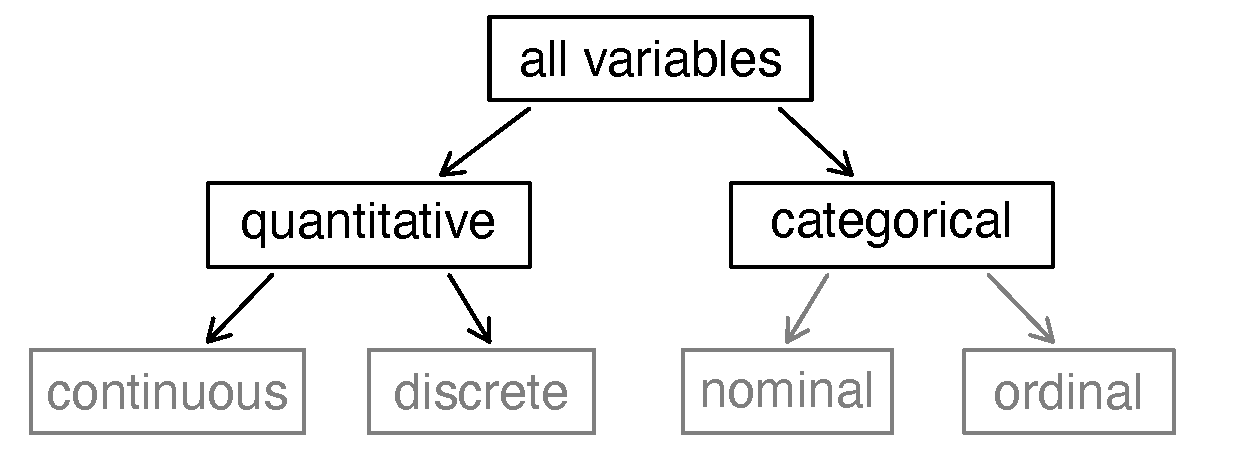
\includegraphics[width=0.6\linewidth]{images/variables} 

}

\caption{Types of variables.}\label{fig:types-of-variables}
\end{figure}

\begin{enumerate}
\def\labelenumi{\arabic{enumi}.}
\setcounter{enumi}{3}
\tightlist
\item
  Is the variable identified in question 3 categorical or quantitative?
\end{enumerate}

\vspace{0.3in}

\begin{enumerate}
\def\labelenumi{\arabic{enumi}.}
\setcounter{enumi}{4}
\tightlist
\item
  Were you correct or incorrect in identifying Bumba?
\end{enumerate}

\vspace{0.3in}

\newpage

\textbf{Step 3}: Once we have collected data, the next step is to \emph{summarize and visualize the data}.

\begin{enumerate}
\def\labelenumi{\arabic{enumi}.}
\setcounter{enumi}{5}
\tightlist
\item
  How many people in your class were correct in identifying Bumba? Using the class size from question 2, calculate the proportion of students who correctly identified Bumba.
\end{enumerate}

\begin{center}
$\mbox{proportion} = \frac{\mbox{number of students who correctly identified Bumba}}{\mbox{total number of students}}$
\end{center}

\vspace{0.7in}

The proportion in question 6 is called a \textbf{summary statistic}---a single value that summarizes the data set. It is important to note that a variable is different than a summary statistic. A \emph{variable} is measured on a \emph{single observational unit} while a summary statistic is calculated from a group of observational units. For example, the variable ``whether or not a student lives on campus'' can be measured on each individual student. In a class of 50 students we can calculate the proportion of students who live on campus, the summary statistic. Look back and make sure you wrote the variable in question 3 as a variable, NOT a summary statistic.

Looking at the data set and the summary statistics is only one way to display the data. We will also want to create a visualization or picture of the data. A \textbf{frequency bar plot} is used to display categorical data as a count or frequency. Since our variable has two levels, correct or incorrect, we will create two bars---one for each level.

\begin{enumerate}
\def\labelenumi{\arabic{enumi}.}
\setcounter{enumi}{6}
\tightlist
\item
  Plot the observed class data using a frequency bar plot. Be sure to add a scale to the y-axis.
\end{enumerate}

\begin{center}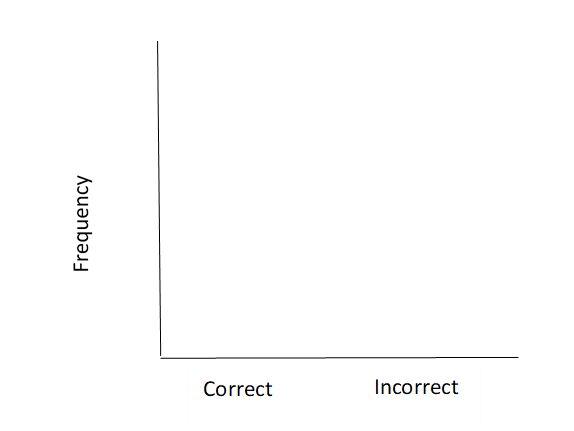
\includegraphics[width=0.4\linewidth]{images/barplot_martian} \end{center}

We can also visualize the data as a proportion in a \textbf{relative frequency bar plot}. Relative frequency is the proportion calculated for each level of the categorical variable.

\begin{enumerate}
\def\labelenumi{\arabic{enumi}.}
\setcounter{enumi}{7}
\tightlist
\item
  Plot the observed class data using a relative frequency bar plot. Be sure to add a scale to the y-axis.
\end{enumerate}

\begin{center}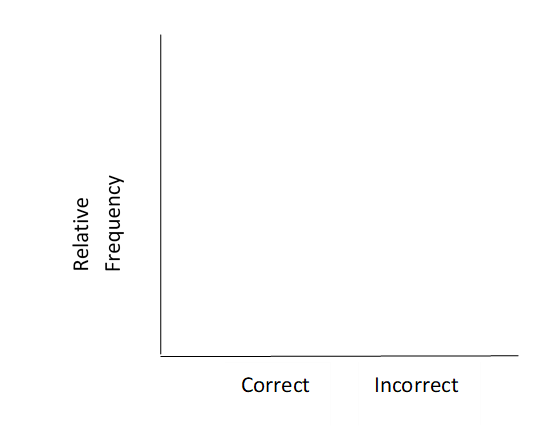
\includegraphics[width=0.4\linewidth]{images/relative_barplot_martian} \end{center}

\newpage

\textbf{Step 4}: The next step is to \emph{use statistical analysis methods to draw inferences from the data}. To answer the research question, we will simulate what \emph{could} have happened in our class given random chance, repeat that many times to understand the expected \emph{variability} between different ``randomly guessing'' classes, then compare our class's observed data to the simulation. This gives us an estimate of how often (or the probability of) our class's result would occur if we were all merely guessing, allowing us to determine if the data provides evidence that we as a class can in fact read Martian.

\begin{enumerate}
\def\labelenumi{\arabic{enumi}.}
\setcounter{enumi}{8}
\item
  If humans really don't know Martian and are just guessing which is Bumba, what are the chances of getting it right?
  \vspace{0.3in}

  How could we use a coin to simulate each student ``just guessing'' which Martian letter is Bumba?
  \vspace{.9in}

  How could we use coins to simulate the entire class ``just guessing'' which Martian letter is Bumba?
  \vspace{.9in}

  How many people in your class would you expect to choose Bumba correctly just by chance? Explain your reasoning.
  \vspace{.9in}
\item
  Each of you will flip a coin one time to simulate your ``guess''. Let Heads = correct, Tails = incorrect. What was the result of your simulation?
  \vspace{.3in}

  What was the result from your class's simulation? What proportion of students ``guessed'' correctly in the simulation?
  \vspace{.3in}
\item
  If students really don't know Martian and are just guessing which is Bumba, which seems more unusual: the result from your class's \textbf{simulation} or the observed proportion of students in your class that were correct (this is your summary statistic from question 6)? Explain your reasoning.
\end{enumerate}

\newpage

\begin{enumerate}
\def\labelenumi{\arabic{enumi}.}
\setcounter{enumi}{11}
\tightlist
\item
  While your observed class data is likely far different from the simulated ``just-guessing'' class, comparing our class data to a single simulation does not seem to give enough information. The differences seen could just be due to that set of coin flips! Let's simulate another class. Each student should flip your coin again. What was the result from your class's second simulation? What proportion of students ``guessed'' correctly in the second simulation? Create a plot to compare the two simulated results with the observed class result.
\end{enumerate}

\vspace{1in}

\begin{enumerate}
\def\labelenumi{\arabic{enumi}.}
\setcounter{enumi}{12}
\tightlist
\item
  We still unfortunately only have a couple of simulations to compare our class data to. It would be much better to be able to see how our class compared to hundreds or thousands of ``just-guessing'' classes. Since we don't want to flip coins all class period, your instructor will use a computer simulation to get 1000 trials. Fill in the following blanks to describe how we would create a simulation of random guessing with 1000 trials.
\end{enumerate}

~~~~~~~~~~Probability of correct guesses: \_\_\_\_\_

\vspace{0.05in}

~~~~~~~~~~Sample size: \_\_\_\_\_

\vspace{0.05in}

~~~~~~~~~~Number of repetitions: \_\_\_\_\_

\vspace{0.05in}

\begin{enumerate}
\def\labelenumi{\arabic{enumi}.}
\setcounter{enumi}{13}
\tightlist
\item
  Sketch the distribution displayed by your instructor here, being sure to label each axis appropriately.
\end{enumerate}

\vspace{1.5in}

\begin{enumerate}
\def\labelenumi{\arabic{enumi}.}
\setcounter{enumi}{14}
\tightlist
\item
  Is your class particularly good or bad at Martian? How can you use the plot in question 14 to tell?
\end{enumerate}

\vspace{.8in}

\begin{enumerate}
\def\labelenumi{\arabic{enumi}.}
\setcounter{enumi}{15}
\tightlist
\item
  Is it \emph{possible} that we could see our class results just by chance if everyone was just guessing? Explain your reasoning.
\end{enumerate}

\vspace{.5in}

\begin{enumerate}
\def\labelenumi{\arabic{enumi}.}
\setcounter{enumi}{16}
\tightlist
\item
  Is it \emph{likely} that we could see our class results just by chance if everyone was just guessing? Explain your reasoning.
\end{enumerate}

\vspace{.5in}

\newpage

\textbf{Step 5}: The next step in the statistical investigation process is to \emph{communicate the results and answer the research question}.

\begin{enumerate}
\def\labelenumi{\arabic{enumi}.}
\setcounter{enumi}{17}
\tightlist
\item
  Does this activity provide strong evidence that students were not just guessing at random? If so, what do you think is going on here? Can we as a class read Martian?\footnote{Reference for ``Martian alphabet'' is a TED talk given by Vilayanur Ramachandran in 2007. The synesthesia part begins at roughly 17:30 minutes: \texttt{http://www.ted.com/talks/vilayanur\_ramachandran\_on\_your\_mind}.}
\end{enumerate}

\vspace{1in}

\textbf{Step 6}: The final step of any statistical investigation is to \emph{revisit and look ahead}.

\begin{enumerate}
\def\labelenumi{\arabic{enumi}.}
\setcounter{enumi}{18}
\tightlist
\item
  Can you think of any limitations of our study? Can you think of a new topic that might be on interest based on the results of our study?
\end{enumerate}

\vspace{1in}

\hypertarget{take-home-messages}{%
\section{Take home messages}\label{take-home-messages}}

\begin{enumerate}
\def\labelenumi{\arabic{enumi}.}
\item
  In this course we will learn how to evaluate a claim by comparing observed results (classes' ``guesses'' when asked to identify Bumba) to a distribution of many simulated results under an assumption like ``blind guessing.''
\item
  Blind guessing between two outcomes will be correct only about half the time. We can create data (via computer simulation) to fit the assumption of blind guessing.
\item
  Unusual observed results will make us doubt the assumptions used to create the simulated distribution. A large number of correct ``guesses'' is evidence that a person was not just blindly guessing.
\end{enumerate}

\hypertarget{additional-notes}{%
\section{Additional notes}\label{additional-notes}}

Use this space to summarize your thoughts and take additional notes on today's activity, and to write down the names and contact information of your team mates.

\hypertarget{study-design}{%
\chapter{Study Design}\label{study-design}}

\hypertarget{learning-outcomes}{%
\section{Learning outcomes}\label{learning-outcomes}}

\begin{itemize}
\item
  Explain the purpose of random sampling and its effect on scope of inference
\item
  Explain the purpose of random assignment and its effect on scope of inference
\item
  Identify whether a study is observational or an experiment
\item
  Identify confounding variables in observational studies and explain why they are confounding
\item
  Identify the types of bias present in a study
\end{itemize}

\hypertarget{terminology-review}{%
\section{Terminology review}\label{terminology-review}}

In today's activity, we will examine different types of sampling bias and study designs, confounding variables, and how to determine the scope of inference for a study. Some terms covered in this activity are:

\begin{itemize}
\item
  Population
\item
  Sample
\item
  Parameter
\item
  Statistic
\item
  Selection bias
\item
  Response bias
\item
  Non-response bias
\item
  Scope of inference
\item
  Explanatory variable
\item
  Response variable
\item
  Confounding variable
\item
  Experiment
\item
  Observational study
\end{itemize}

To review these concepts, see Sections 1.3 through 1.6 in the textbook.

\newpage

\hypertarget{types-of-sampling-bias}{%
\section{Types of sampling bias}\label{types-of-sampling-bias}}

There are two parts to study design: how the sample was selected and how the study was conducted. First, we will look at sampling and types of bias (selection, non-response, or response).

In these next questions, identify the target population, the sample, the variable, and the type of bias present.

\begin{enumerate}
\def\labelenumi{\arabic{enumi}.}
\item
  To determine if the proportion of out-of-state undergraduate students at Montana State University has increased in the last 10 years, a statistics instructor sent an email survey to 500 randomly selected current undergraduate students. One of the questions on the survey asked whether they had in-state or out-of-state residency. She only received 378 responses.
  \vspace{0.25in}

  Target population:
  \vspace{0.3in}

  Sample:
  \vspace{0.3in}

  Variable:
  \vspace{0.3in}

  Type(s) of bias:
  \vspace{0.3in}
\item
  Pew Research surveys US adults about many different topics. Recently, a survey was conducted to assess current presidential approval. A random sample of 6395 US adults was taken. Of those surveyed, 42\% said they agree with President Trump on many or nearly all of the top issues facing the country today.
  \vspace{0.25in}

  Target population:
  \vspace{0.3in}

  Sample:
  \vspace{0.3in}

  Variable:
  \vspace{0.3in}

  Type(s) of bias:
  \vspace{0.3in}
\end{enumerate}

\newpage

\begin{enumerate}
\def\labelenumi{\arabic{enumi}.}
\setcounter{enumi}{2}
\item
  A television station is interested in predicting whether or not a local referendum to legalize marijuana for adult use will pass. It asks its viewers to phone in and indicate whether they are in favor or opposed to the referendum. Of the 2241 viewers who phoned in, forty-five percent were opposed to legalizing marijuana.
  \vspace{0.1in}

  Target population:
  \vspace{0.3in}

  Sample:
  \vspace{0.3in}

  Variable:
  \vspace{0.3in}

  Type(s) of bias:
  \vspace{0.3in}
\item
  To gauge the interest in a new swimming pool, a local organization stood outside of the Bogart Pool during open hours. One of the questions they asked was, ``Since the Bogart Pool is in such bad repair, don't you agree that the city should fund a new pool?''
  \vspace{0.1in}

  Target population:
  \vspace{0.3in}

  Sample:
  \vspace{0.3in}

  Variable:
  \vspace{0.3in}

  Type(s) of bias:
  \vspace{0.3in}
\item
  The Bozeman school district is interested in surveying parents of students about their opinions on returning to school this fall following the COVID-19 pandemic. They divided the school district into 10 divisions based on location and randomly surveyed 20 households within each division.
  \vspace{0.1in}

  Target population:
  \vspace{0.3in}

  Sample:
  \vspace{0.3in}

  Variable:
  \vspace{0.3in}

  Type(s) of bias:
  \vspace{0.3in}
\end{enumerate}

\newpage

\hypertarget{study-design-1}{%
\section{Study design}\label{study-design-1}}

The two main study designs we will cover are \textbf{observational studies} and \textbf{experiments}. Both the sampling method and the study design will help to determine the \textbf{scope of inference} for a study. Remember that only in a randomized experiment can we conclude a \textbf{causal} (cause and effect) relationship between the explanatory and response variable.

\begin{center}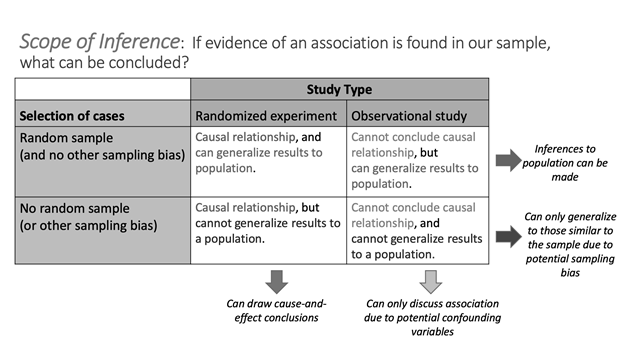
\includegraphics[width=0.75\linewidth]{images/ScopeOfInferenceGreyscale} \end{center}

For the next exercises, identify the explanatory variable, the response variable, the study design (observational study or experiment), and the scope of inference.

\begin{enumerate}
\def\labelenumi{\arabic{enumi}.}
\setcounter{enumi}{5}
\item
  The pharmaceutical company Moderna Therapeutics is working in conjunction with the National Institutes of Health towards a vaccine for COVID-19 and has recently begun Phase 3 clinical trials. US clinical research sites will enroll 30,000 volunteers without COVID-19 to participate. Participants will be randomly assigned to receive either the candidate vaccine or a saline placebo. They will then be followed to assess vaccine-related symptoms and development of COVID-19. The trial is double-blind, so neither the investigators nor the participants will know who is assigned to which group.
  \vspace{0.1in}

  Explanatory variable:
  \vspace{0.25in}

  Response variable:
  \vspace{0.25in}

  Study design:
  \vspace{0.25in}

  What is the scope of inference for this study?
  \vspace{0.5in}
\end{enumerate}

\newpage

\begin{enumerate}
\def\labelenumi{\arabic{enumi}.}
\setcounter{enumi}{6}
\item
  In another study, a local health department randomly selected 1000 US adults without COVID-19 to participate in a health survey. Each participant was assessed at the beginning of the study and then followed for one year. They were interested to see which participants elected to receive a vaccination for COVID-19 and whether any participants developed COVID-19.
  \vspace{0.1in}

  Explanatory variable:
  \vspace{0.25in}

  Response vnariable:
  \vspace{0.25in}

  Study design:
  \vspace{0.25in}

  What is the scope of inference for this study?
  \vspace{0.5in}
\item
  For each of the studies in questions 6 and 7, determine whether confounding variables could be an issue. If so, identify a potential confounding variable and explain how it meets the definition of a confounding variable.
  \vspace{1.5in}
\end{enumerate}

\hypertarget{additional-notes}{%
\section{Additional notes}\label{additional-notes}}

Use this space to summarize your thoughts and take additional notes on today's activity.

\hypertarget{current-population-survey}{%
\chapter{Current Population Survey}\label{current-population-survey}}

\hypertarget{learning-outcomes}{%
\section{Learning outcomes}\label{learning-outcomes}}

\begin{itemize}
\item
  Identify and create appropriate summary statistics and plots
  given a data set or research question
\item
  Plots for a single categorical variable: bar plot
\item
  Plots for association between two categorical variables:
  segmented bar plot, mosaic plot
\item
  Recognize and simulate probabilities as long-run frequencies
\item
  Construct two-way tables to evaluate conditional probabilities
\end{itemize}

\hypertarget{terminology-review}{%
\section{Terminology review}\label{terminology-review}}

In today's activity, we will review summary measures and plots for categorical variables. Some terms covered in this activity are:

\begin{itemize}
\item
  Proportions
\item
  Bar plots
\item
  Segmented bar plots
\item
  Probability
\item
  Conditional probability
\item
  Two-way tables
\end{itemize}

To review these concepts, see Sections 2.1 and 2.2 in the textbook.

\newpage

\hypertarget{current-population-survey-1985}{%
\section{``Current'' Population Survey: 1985}\label{current-population-survey-1985}}

The data set we will use for this activity is from the Current Population Survey (CPS) in 1985. The CPS is a survey sponsored by the Census Bureau and the Bureau of Labor Statistics to track labor force statistics for the United States population. The following table describes the variables in the data set:

\begin{longtable}[]{@{}ll@{}}
\toprule
\begin{minipage}[b]{0.11\columnwidth}\raggedright
\textbf{Variable}\strut
\end{minipage} & \begin{minipage}[b]{0.83\columnwidth}\raggedright
\textbf{Description}\strut
\end{minipage}\tabularnewline
\midrule
\endhead
\begin{minipage}[t]{0.11\columnwidth}\raggedright
\texttt{educ}\strut
\end{minipage} & \begin{minipage}[t]{0.83\columnwidth}\raggedright
Number of years of education\strut
\end{minipage}\tabularnewline
\begin{minipage}[t]{0.11\columnwidth}\raggedright
\texttt{south}\strut
\end{minipage} & \begin{minipage}[t]{0.83\columnwidth}\raggedright
Whether lives in southern region of the US: \texttt{S} = lives in south, \texttt{NS} = does not live in south\strut
\end{minipage}\tabularnewline
\begin{minipage}[t]{0.11\columnwidth}\raggedright
\texttt{sex}\strut
\end{minipage} & \begin{minipage}[t]{0.83\columnwidth}\raggedright
Sex: \texttt{M} = male, \texttt{F} = female\strut
\end{minipage}\tabularnewline
\begin{minipage}[t]{0.11\columnwidth}\raggedright
\texttt{exper}\strut
\end{minipage} & \begin{minipage}[t]{0.83\columnwidth}\raggedright
Number of years of work experience (inferred from age and education)\strut
\end{minipage}\tabularnewline
\begin{minipage}[t]{0.11\columnwidth}\raggedright
\texttt{union}\strut
\end{minipage} & \begin{minipage}[t]{0.83\columnwidth}\raggedright
Whether union member: \texttt{Union} or \texttt{Not}\strut
\end{minipage}\tabularnewline
\begin{minipage}[t]{0.11\columnwidth}\raggedright
\texttt{wage}\strut
\end{minipage} & \begin{minipage}[t]{0.83\columnwidth}\raggedright
Wage (dollars per hour) \textbar{}\strut
\end{minipage}\tabularnewline
\begin{minipage}[t]{0.11\columnwidth}\raggedright
\texttt{age}\strut
\end{minipage} & \begin{minipage}[t]{0.83\columnwidth}\raggedright
Age (years)\strut
\end{minipage}\tabularnewline
\begin{minipage}[t]{0.11\columnwidth}\raggedright
\texttt{race}\strut
\end{minipage} & \begin{minipage}[t]{0.83\columnwidth}\raggedright
Race: \texttt{W} = white, \texttt{NW} = not white \textbar{}\strut
\end{minipage}\tabularnewline
\begin{minipage}[t]{0.11\columnwidth}\raggedright
\texttt{sector}\strut
\end{minipage} & \begin{minipage}[t]{0.83\columnwidth}\raggedright
Sector of the economy: \texttt{clerical}, \texttt{const} (construction), \texttt{management}, \texttt{manufacturing}, \texttt{professional}, \texttt{sales}, \texttt{service}, \texttt{other}\strut
\end{minipage}\tabularnewline
\begin{minipage}[t]{0.11\columnwidth}\raggedright
\texttt{married}\strut
\end{minipage} & \begin{minipage}[t]{0.83\columnwidth}\raggedright
Marital status: \texttt{Married} or \texttt{Single}\strut
\end{minipage}\tabularnewline
\bottomrule
\end{longtable}

\hypertarget{vocabulary-review}{%
\subsection{Vocabulary review}\label{vocabulary-review}}

\begin{enumerate}
\def\labelenumi{\arabic{enumi}.}
\tightlist
\item
  What are the observational units?
\end{enumerate}

\vspace{0.2in}

\begin{enumerate}
\def\labelenumi{\arabic{enumi}.}
\setcounter{enumi}{1}
\tightlist
\item
  Which variables are categorical?
\end{enumerate}

\vspace{0.4in}

\begin{enumerate}
\def\labelenumi{\arabic{enumi}.}
\setcounter{enumi}{2}
\tightlist
\item
  What types of plots can be used to display categorical data?
\end{enumerate}

\vspace{0.5in}

An important part of understanding data is to create visual pictures of what the data represent. In this activity, we will create graphical representations of categorical data.

\hypertarget{r-code}{%
\subsection{\texorpdfstring{\texttt{R} code}{R code}}\label{r-code}}

\texttt{R} is a free statistical analysis software program we will use in Stat 216. Please see D2L for instructions on how to download or
access a version of \texttt{R} on your laptop, or plan to use the school computers for some parts of assigned out of class work for this course.

Throughout these activities, we will often include the \texttt{R} code
you would use in order to produce output or plots. These
``code chunks'' appear in gray. In the code chunk below, we
demonstrate how to read the data set into \texttt{R} using the \texttt{read.csv()} function, and tell \texttt{R} to treat the \texttt{sector} and \texttt{sex} variables as categorical variables (``factors'').

The \# sign is not part of the \texttt{R} code.
It is used by these authors to add comments to the \texttt{R} code and explain what each call is telling the program to do.

\begin{Shaded}
\begin{Highlighting}[]
\NormalTok{cps \textless{}{-}}\StringTok{ }\KeywordTok{read.csv}\NormalTok{(}\StringTok{"data/cps.csv"}\NormalTok{) }\CommentTok{\#This will read in the data set}
\end{Highlighting}
\end{Shaded}

\hypertarget{displaying-a-single-categorical-variable}{%
\subsection{Displaying a single categorical variable}\label{displaying-a-single-categorical-variable}}

If we wanted to know how many people in our data set were in each sector, we would create a frequency bar plot of the variable \texttt{sector}.

\begin{Shaded}
\begin{Highlighting}[]
\NormalTok{cps }\OperatorTok{\%\textgreater{}\%}\StringTok{ }\CommentTok{\#Data set piped into...}
\KeywordTok{ggplot}\NormalTok{(}\KeywordTok{aes}\NormalTok{(}\DataTypeTok{y =}\NormalTok{ sector)) }\OperatorTok{+}\StringTok{   }\CommentTok{\#This specifies the variable}
\StringTok{  }\KeywordTok{geom\_bar}\NormalTok{(}\DataTypeTok{stat =} \StringTok{"count"}\NormalTok{) }\OperatorTok{+}\StringTok{  }\CommentTok{\#Tell it to make a bar plot}
\StringTok{  }\KeywordTok{labs}\NormalTok{(}\DataTypeTok{title =} \StringTok{"Frequency Bar Plot of Sector"}\NormalTok{,  }\CommentTok{\#Give your plot a title}
       \DataTypeTok{x =} \StringTok{"Frequency"}\NormalTok{,   }\CommentTok{\#Label the x axis}
       \DataTypeTok{y =} \StringTok{"Sector"}\NormalTok{)  }\OperatorTok{+}\StringTok{ }\CommentTok{\#Label the y axis}
\StringTok{  }\KeywordTok{coord\_flip}\NormalTok{()  }\CommentTok{\#Turn the bars so they are vertical}
\end{Highlighting}
\end{Shaded}

\begin{center}\includegraphics[width=0.5\linewidth]{03-EDA-categorical_files/figure-latex/unnamed-chunk-2-1} \end{center}

\begin{enumerate}
\def\labelenumi{\arabic{enumi}.}
\setcounter{enumi}{3}
\tightlist
\item
  Which sector of the economy has the largest number of people in it? Approximately how many people are in this sector?
\end{enumerate}

\vspace{0.3in}

We could also choose to display the data as a proportion in a relative frequency bar plot. To find the relative frequency, divide the count in each sector by the sample size. These are sample proportions.

\begin{Shaded}
\begin{Highlighting}[]
\NormalTok{cps }\OperatorTok{\%\textgreater{}\%}\StringTok{ }\CommentTok{\#Data set piped into...}
\KeywordTok{ggplot}\NormalTok{(}\KeywordTok{aes}\NormalTok{(}\DataTypeTok{x =}\NormalTok{ sector)) }\OperatorTok{+}\StringTok{   }\CommentTok{\#This specifies the variable}
\StringTok{  }\KeywordTok{geom\_bar}\NormalTok{(}\KeywordTok{aes}\NormalTok{(}\DataTypeTok{y =}\NormalTok{ ..prop.., }\DataTypeTok{group =} \DecValTok{1}\NormalTok{)) }\OperatorTok{+}\StringTok{  }\CommentTok{\#Tell it to make a bar plot with proportions}
\StringTok{  }\KeywordTok{labs}\NormalTok{(}\DataTypeTok{title =} \StringTok{"Relative Frequency Bar Plot of Sector"}\NormalTok{,  }\CommentTok{\#Give your plot a title}
       \DataTypeTok{x =} \StringTok{"Sector"}\NormalTok{,   }\CommentTok{\#Label the x axis}
       \DataTypeTok{y =} \StringTok{"Relative Frequency"}\NormalTok{)  }\CommentTok{\#Label the y axis}
\end{Highlighting}
\end{Shaded}

\begin{center}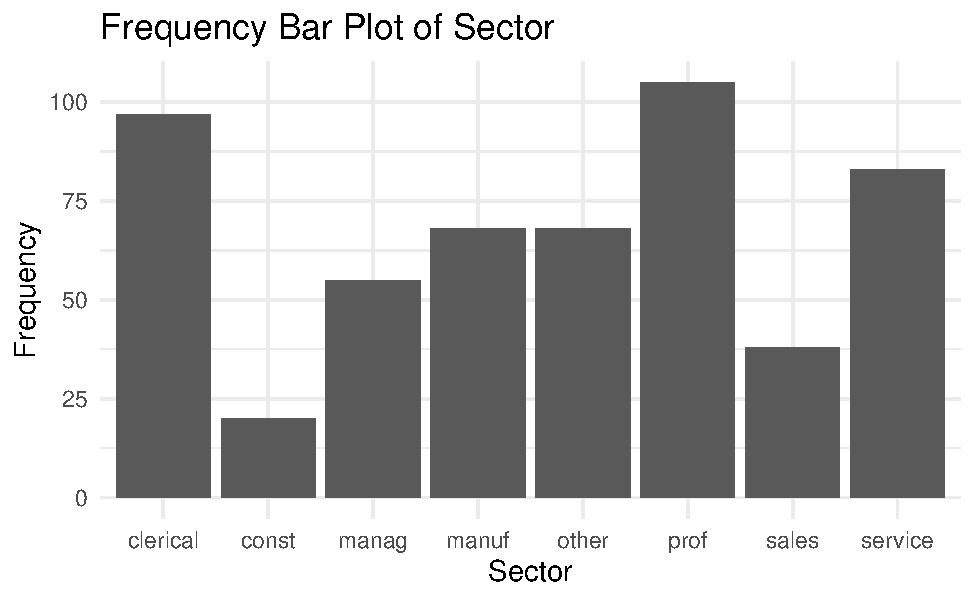
\includegraphics[width=0.5\linewidth]{03-EDA-categorical_files/figure-latex/unnamed-chunk-3-1} \end{center}

\begin{enumerate}
\def\labelenumi{\arabic{enumi}.}
\setcounter{enumi}{4}
\tightlist
\item
  Which features in the relative frequency bar plot are the same as the frequency bar plot? Which are different?
\end{enumerate}

\vspace{1in}

\hypertarget{displaying-two-categorical-variables}{%
\subsection{Displaying two categorical variables}\label{displaying-two-categorical-variables}}

To examine the differences proportion of males and females across sectors, we would create a segmented bar plot of \texttt{sector} segmented by \texttt{sex}.

\begin{Shaded}
\begin{Highlighting}[]
\NormalTok{cps }\OperatorTok{\%\textgreater{}\%}\StringTok{ }\CommentTok{\#Data set piped into...}
\KeywordTok{ggplot}\NormalTok{(}\KeywordTok{aes}\NormalTok{(}\DataTypeTok{x =}\NormalTok{ sector, }\DataTypeTok{fill =}\NormalTok{ sex)) }\OperatorTok{+}\StringTok{   }\CommentTok{\#This specifies the variables}
\StringTok{  }\KeywordTok{geom\_bar}\NormalTok{(}\DataTypeTok{stat =} \StringTok{"count"}\NormalTok{, }\DataTypeTok{position =} \StringTok{"fill"}\NormalTok{) }\OperatorTok{+}\StringTok{  }\CommentTok{\#Tell it to make a stacked bar plot}
\StringTok{  }\KeywordTok{labs}\NormalTok{(}\DataTypeTok{title =} \StringTok{"Segmented Bar Plot of Sector by Sex"}\NormalTok{,  }\CommentTok{\#Make sure to title your plot }
       \DataTypeTok{x =} \StringTok{"Sector"}\NormalTok{,   }\CommentTok{\#Label the x axis}
       \DataTypeTok{y =} \StringTok{""}\NormalTok{) }\OperatorTok{+}\StringTok{  }\CommentTok{\#Remove y axis label}
\StringTok{    }\KeywordTok{scale\_fill\_grey}\NormalTok{()  }\CommentTok{\#Make figure black and white}
\end{Highlighting}
\end{Shaded}

\begin{center}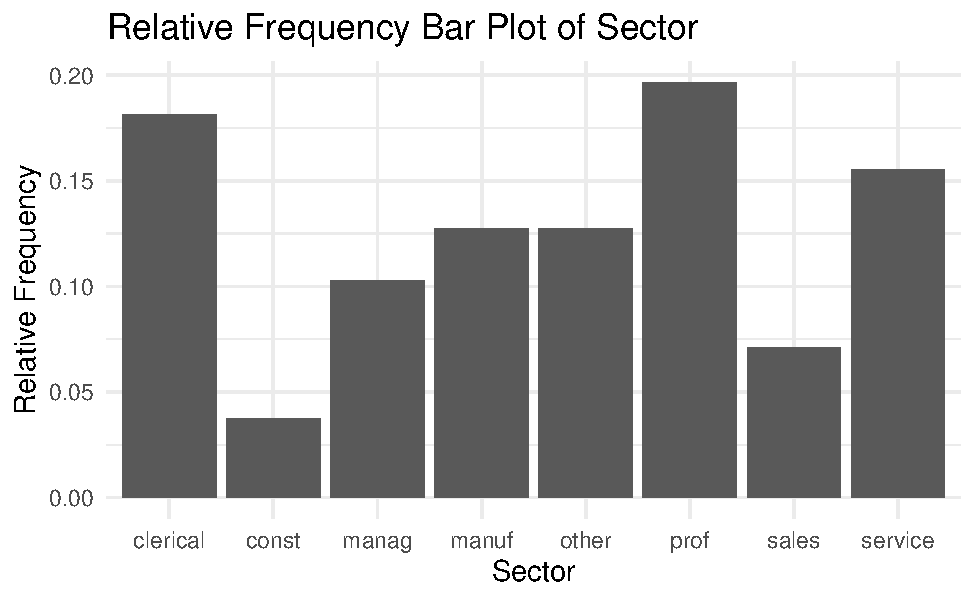
\includegraphics[width=0.6\linewidth]{03-EDA-categorical_files/figure-latex/unnamed-chunk-4-1} \end{center}

\begin{enumerate}
\def\labelenumi{\arabic{enumi}.}
\setcounter{enumi}{5}
\tightlist
\item
  Using the segmented bar plot, which sector has about the same proportion of males and females?
\end{enumerate}

\vspace{0.5in}

\begin{enumerate}
\def\labelenumi{\arabic{enumi}.}
\setcounter{enumi}{6}
\tightlist
\item
  Which sector has the highest proportion of females?
\end{enumerate}

\vspace{0.5in}

\begin{enumerate}
\def\labelenumi{\arabic{enumi}.}
\setcounter{enumi}{7}
\tightlist
\item
  Which variable is the bar plot treating as the explanatory variable? Which is the response variable?
\end{enumerate}

\newpage

\hypertarget{probability}{%
\section{Probability}\label{probability}}

\begin{enumerate}
\def\labelenumi{\arabic{enumi}.}
\setcounter{enumi}{8}
\item
  A study was reported in which ninth grade Minnesota teens were asked whether they had gambled at least once a week in the past year. The sample consisted of 49.1\% boys. The proportion of boys who had gambled at least once per week during the past year was 0.229, while among non-boys this proportion was only 0.045.
  \vspace{1mm}

  Let B = the event the person is a boy, and C = the event the person is a weekly gambler.
  \vspace{0.1in}
\end{enumerate}

\begin{enumerate}
\def\labelenumi{\alph{enumi}.}
\item
  Draw a segmented bar plot of sex segmented by gambling. Make sure to clearly label your axes and legend.
  \vspace{1.8in}
\item
  Identify what each numerical value given in the problem represents in probability notation.
  \vspace{.1in}
\end{enumerate}

~~~~~~~~~~~~~~~~0.491 = \vspace{.1in}\\
\hspace*{0.333em}\hspace*{0.333em}\hspace*{0.333em}\hspace*{0.333em}\hspace*{0.333em}\hspace*{0.333em}\hspace*{0.333em}\hspace*{0.333em}\hspace*{0.333em}\hspace*{0.333em}\hspace*{0.333em}\hspace*{0.333em}\hspace*{0.333em}\hspace*{0.333em}\hspace*{0.333em}\hspace*{0.333em}0.229 =

\vspace{.1in}

~~~~~~~~~~~~~~~~0.045 =

\vspace{.1in}

\begin{enumerate}
\def\labelenumi{\alph{enumi}.}
\setcounter{enumi}{2}
\tightlist
\item
  Create a hypothetical two-way table to represent the situation. Recall that in a two-way table, the explanatory variable should be your column headers (similar to the \(x\)-axis in a segmented bar graph!) while the response variable becomes the row headers.
\end{enumerate}

\begin{longtable}[]{@{}llll@{}}
\toprule
\hspace{1in} & \hspace{1in} & \hspace{1in} & Total\tabularnewline
\midrule
\endhead
\hspace{1in} & & &\tabularnewline
\hspace{1in} & & &\tabularnewline
\hspace{1in} & & &\tabularnewline
Total & & & 100,000\tabularnewline
\bottomrule
\end{longtable}

\begin{enumerate}
\def\labelenumi{\alph{enumi}.}
\setcounter{enumi}{3}
\item
  Find \(P(\mbox{B and C})\). What does this probability represent in the context of the problem?
  \vspace{.8in}
\item
  Find the probability that a selected non-gambler is a non-boy. What is the notation used for this probability?
\end{enumerate}

\newpage

\begin{enumerate}
\def\labelenumi{\arabic{enumi}.}
\setcounter{enumi}{9}
\item
  In a computer store, 30\% of the computers in stock are laptops and 70\% are desktops. Five percent of the laptops are on sale, while 10\% of the desktops are on sale.
  \vspace{1mm}

  Let L = the event the computer is a laptop, and S = the event the computer is on sale.
  \vspace{0.1in}
\end{enumerate}

\begin{enumerate}
\def\labelenumi{\alph{enumi}.}
\tightlist
\item
  Identify what each numerical value given in the problem represents in probability notation.
  \vspace{.1in}
\end{enumerate}

~~~~~~~~~~~~~~~~0.30 = \vspace{.1in}\\
\hspace*{0.333em}\hspace*{0.333em}\hspace*{0.333em}\hspace*{0.333em}\hspace*{0.333em}\hspace*{0.333em}\hspace*{0.333em}\hspace*{0.333em}\hspace*{0.333em}\hspace*{0.333em}\hspace*{0.333em}\hspace*{0.333em}\hspace*{0.333em}\hspace*{0.333em}\hspace*{0.333em}\hspace*{0.333em}0.70 =

\vspace{.1in}

~~~~~~~~~~~~~~~~0.05 =

\vspace{.1in}

~~~~~~~~~~~~~~~~0.10 =

\vspace{.1in}

\begin{enumerate}
\def\labelenumi{\alph{enumi}.}
\setcounter{enumi}{1}
\tightlist
\item
  Create a hypothetical two-way table to represent the situation.
\end{enumerate}

\begin{longtable}[]{@{}llll@{}}
\toprule
\hspace{1in} & \hspace{1in} & \hspace{1in} & Total\tabularnewline
\midrule
\endhead
\hspace{1in} & & &\tabularnewline
\hspace{1in} & & &\tabularnewline
\hspace{1in} & & &\tabularnewline
Total & & & 100,000\tabularnewline
\bottomrule
\end{longtable}

\begin{enumerate}
\def\labelenumi{\alph{enumi}.}
\setcounter{enumi}{2}
\item
  Calculate the probability that a randomly selected computer will be a desktop, given that the computer is on sale. What is the notation used for this probability?
  \vspace{.8in}
\item
  Find \(P(S | L^C)\). What does this probability represent in context of the problem?
  \vspace{1in}
\end{enumerate}

\hypertarget{additional-notes}{%
\section{Additional notes}\label{additional-notes}}

Use this space to summarize your thoughts and take additional notes on today's activity.

\hypertarget{imdb-movie-reviews}{%
\chapter{IMDb Movie Reviews}\label{imdb-movie-reviews}}

\hypertarget{learning-objectives}{%
\section{Learning objectives}\label{learning-objectives}}

\begin{itemize}
\item
  Identify and create appropriate summary statistics and plots
  given a data set or research question for quantitative data
\item
  Interpret the following summary statistics in context:
  median, lower quartile, upper quartile,
  standard deviation, inter-quartile range
\item
  Given a plot or set of plots, describe and compare the distribution(s)
  of a single quantitative variable
  (center, variability, shape, outliers)
\end{itemize}

\hypertarget{terminology-review}{%
\section{Terminology review}\label{terminology-review}}

In today's activity, we will review summary measures and plots for quantitative variables. Some terms covered in this activity are:

\begin{itemize}
\item
  Two measures of center: mean, median
\item
  Two measures of spread (variability): standard deviation, inter-quartile range (IQR)
\item
  Types of graphs: box plots, dot plots, histograms
\end{itemize}

To review these concepts, see Section 2.3 in the textbook.

\hypertarget{movies-released-in-2016}{%
\section{Movies released in 2016}\label{movies-released-in-2016}}

A data set was collected on movies released in 2016. Here is a list of some of the variables collected on these movies.

\begin{longtable}[]{@{}ll@{}}
\toprule
\begin{minipage}[b]{0.22\columnwidth}\raggedright
\textbf{Variable}\strut
\end{minipage} & \begin{minipage}[b]{0.72\columnwidth}\raggedright
\textbf{Description}\strut
\end{minipage}\tabularnewline
\midrule
\endhead
\begin{minipage}[t]{0.22\columnwidth}\raggedright
\texttt{budget\_mil}\strut
\end{minipage} & \begin{minipage}[t]{0.72\columnwidth}\raggedright
Amount of money (in US \$ millions) budgeted for the production of the movie\strut
\end{minipage}\tabularnewline
\begin{minipage}[t]{0.22\columnwidth}\raggedright
\texttt{revenue\_mil}\strut
\end{minipage} & \begin{minipage}[t]{0.72\columnwidth}\raggedright
Amount of money (in US \$ millions) the movie made after release\strut
\end{minipage}\tabularnewline
\begin{minipage}[t]{0.22\columnwidth}\raggedright
\texttt{duration}\strut
\end{minipage} & \begin{minipage}[t]{0.72\columnwidth}\raggedright
Length of the movie (in minutes)\strut
\end{minipage}\tabularnewline
\begin{minipage}[t]{0.22\columnwidth}\raggedright
\texttt{content\_rating}\strut
\end{minipage} & \begin{minipage}[t]{0.72\columnwidth}\raggedright
Rating of the movie (\texttt{G}, \texttt{PG}, \texttt{PG-13}, \texttt{R}, \texttt{Not\ Rated})\strut
\end{minipage}\tabularnewline
\begin{minipage}[t]{0.22\columnwidth}\raggedright
\texttt{imdb\_score}\strut
\end{minipage} & \begin{minipage}[t]{0.72\columnwidth}\raggedright
IMDb user rating score from 1 to 10\strut
\end{minipage}\tabularnewline
\begin{minipage}[t]{0.22\columnwidth}\raggedright
\texttt{genres}\strut
\end{minipage} & \begin{minipage}[t]{0.72\columnwidth}\raggedright
Categories the movie falls into (e.g., Action, Drama, etc.)\strut
\end{minipage}\tabularnewline
\begin{minipage}[t]{0.22\columnwidth}\raggedright
\texttt{movie\_facebook\_likes}\strut
\end{minipage} & \begin{minipage}[t]{0.72\columnwidth}\raggedright
Number of likes a movie receives on Facebook\strut
\end{minipage}\tabularnewline
\bottomrule
\end{longtable}

\newpage

\hypertarget{vocabulary-review}{%
\subsection{Vocabulary review}\label{vocabulary-review}}

\begin{enumerate}
\def\labelenumi{\arabic{enumi}.}
\tightlist
\item
  What are the observational units in this data set?
\end{enumerate}

\vspace{0.3in}

\begin{enumerate}
\def\labelenumi{\arabic{enumi}.}
\setcounter{enumi}{1}
\tightlist
\item
  Which of the above listed variables are categorical?
\end{enumerate}

\vspace{.5in}

\begin{enumerate}
\def\labelenumi{\arabic{enumi}.}
\setcounter{enumi}{2}
\tightlist
\item
  Which of the above listed variables are quantitative?
\end{enumerate}

\vspace{.5in}

\hypertarget{summarizing-a-single-quantitative-variable}{%
\subsection{Summarizing a single quantitative variable}\label{summarizing-a-single-quantitative-variable}}

The \texttt{favstats} function gives the summary statistics for a quantitative variable. Here we have the summary statistics for the variable \texttt{imdb\_score}.

\begin{Shaded}
\begin{Highlighting}[]
\NormalTok{movies \textless{}{-}}\StringTok{ }\KeywordTok{read.csv}\NormalTok{(}\StringTok{"data/Movies2016.csv"}\NormalTok{) }\CommentTok{\# Read in data set}
\NormalTok{movies }\OperatorTok{\%\textgreater{}\%}\StringTok{ }\CommentTok{\#Data set piped into...}
\StringTok{  }\KeywordTok{summarise}\NormalTok{(}\KeywordTok{favstats}\NormalTok{(imdb\_score)) }\CommentTok{\#Apply favstats function to imdb\_score}
\end{Highlighting}
\end{Shaded}

\begin{verbatim}
#>   min   Q1 median  Q3 max     mean       sd  n missing
#> 1 3.4 5.65    6.4 7.1 8.2 6.309783 1.086689 92       0
\end{verbatim}

\begin{enumerate}
\def\labelenumi{\arabic{enumi}.}
\setcounter{enumi}{3}
\tightlist
\item
  Give the values for the two measures of center.
\end{enumerate}

\vspace{0.5in}

\begin{enumerate}
\def\labelenumi{\arabic{enumi}.}
\setcounter{enumi}{4}
\tightlist
\item
  Calculate the IQR.
\end{enumerate}

\vspace{0.5in}

\begin{enumerate}
\def\labelenumi{\arabic{enumi}.}
\setcounter{enumi}{5}
\tightlist
\item
  Report the value of the standard deviation and interpret this value in context of the problem.
  \vspace{1in}
\end{enumerate}

\hypertarget{displaying-a-single-quantitative-variable}{%
\subsection{Displaying a single quantitative variable}\label{displaying-a-single-quantitative-variable}}

\begin{enumerate}
\def\labelenumi{\arabic{enumi}.}
\setcounter{enumi}{6}
\tightlist
\item
  What are the three types of plots used to plot a single quantitative variable?
\end{enumerate}

\newpage

A histogram of the variable `IMDb Score' is shown below. Notice that the bin width is 0.5. For example the first bin consists of the number of movies in the data set with an IMDb score of 3.25 to 3.75. It is important to note that a movie with a IMDb score of 4.75 will fall into the bin for 4.75 - 5.25. Visually this shows us the range of IMDb scores for Movies released in 2016.

\begin{Shaded}
\begin{Highlighting}[]
\NormalTok{movies }\OperatorTok{\%\textgreater{}\%}\StringTok{ }\CommentTok{\#Data set piped into...}
\KeywordTok{ggplot}\NormalTok{(}\KeywordTok{aes}\NormalTok{(}\DataTypeTok{x =}\NormalTok{ imdb\_score)) }\OperatorTok{+}\StringTok{   }\CommentTok{\#Name variable to plot}
\StringTok{  }\KeywordTok{geom\_histogram}\NormalTok{(}\DataTypeTok{binwidth =} \FloatTok{0.5}\NormalTok{) }\OperatorTok{+}\StringTok{  }\CommentTok{\#Create histogram with specified binwidth}
\StringTok{  }\KeywordTok{labs}\NormalTok{(}\DataTypeTok{title =} \StringTok{"Histogram of IMDb Score of Movies in 2016"}\NormalTok{, }\CommentTok{\#title for plot}
       \DataTypeTok{x =} \StringTok{"IMDb Score"}\NormalTok{, }\CommentTok{\#Label for x axis}
       \DataTypeTok{y =} \StringTok{"Frequency"}\NormalTok{) }\CommentTok{\#Label for y axis}
\end{Highlighting}
\end{Shaded}

\begin{center}\includegraphics[width=0.6\linewidth]{04-EDA-quantitative_files/figure-latex/unnamed-chunk-2-1} \end{center}

\begin{enumerate}
\def\labelenumi{\arabic{enumi}.}
\setcounter{enumi}{7}
\tightlist
\item
  Which range of IMDb scores have the highest frequency?
\end{enumerate}

\vspace{0.4in}

\begin{enumerate}
\def\labelenumi{\arabic{enumi}.}
\setcounter{enumi}{8}
\tightlist
\item
  What is the shape of the distribution of IMDb scores?
\end{enumerate}

\vspace{0.4in}

\begin{enumerate}
\def\labelenumi{\arabic{enumi}.}
\setcounter{enumi}{9}
\tightlist
\item
  Which five summary statistics are used in creating a box plot? (Hint: Together they are called the \textbf{five-number summary} of the variable.)
\end{enumerate}

\vspace{0.4in}

\begin{enumerate}
\def\labelenumi{\arabic{enumi}.}
\setcounter{enumi}{10}
\item
  The three smallest IMDb scores in the data set are 3.4, 3.5, and 3.7 and the three largest IMDb scores are 8.5, 8.7, and 9.1:

\begin{Shaded}
\begin{Highlighting}[]
\NormalTok{movies }\OperatorTok{\%\textgreater{}\%}\StringTok{ }\CommentTok{\# Data set pipes into...}
\StringTok{  }\KeywordTok{select}\NormalTok{(imdb\_score) }\OperatorTok{\%\textgreater{}\%}\StringTok{ }\CommentTok{\# Select imdb\_score variable}
\StringTok{  }\KeywordTok{slice\_min}\NormalTok{(imdb\_score, }\DataTypeTok{n =} \DecValTok{3}\NormalTok{)  }\CommentTok{\# Show 3 smallest values}
\end{Highlighting}
\end{Shaded}

\begin{verbatim}
#>   imdb_score
#> 1        3.4
#> 2        3.5
#> 3        3.7
\end{verbatim}

  \newpage

\begin{Shaded}
\begin{Highlighting}[]
\NormalTok{movies }\OperatorTok{\%\textgreater{}\%}\StringTok{ }\CommentTok{\# Data set pipes into...}
\StringTok{  }\KeywordTok{select}\NormalTok{(imdb\_score) }\OperatorTok{\%\textgreater{}\%}\StringTok{ }\CommentTok{\# Select imdb\_score variable}
\StringTok{  }\KeywordTok{slice\_max}\NormalTok{(imdb\_score, }\DataTypeTok{n =} \DecValTok{3}\NormalTok{)  }\CommentTok{\# Show 3 largest values}
\end{Highlighting}
\end{Shaded}

\begin{verbatim}
#>   imdb_score
#> 1        8.2
#> 2        8.1
#> 3        8.0
\end{verbatim}

  Using the summary statistics above, and the smallest and largest values of variable to check for outliers, sketch a box plot of IMDb Score. Be sure to label the axes.
\end{enumerate}

\vspace{1.5in}

\hypertarget{displaying-a-single-categorical-and-single-quantitative-variable}{%
\subsection{Displaying a single categorical and single quantitative variable}\label{displaying-a-single-categorical-and-single-quantitative-variable}}

The box plot of `Budget' in millions by `Content rating' is plotted using the code below. This plot helps to compare the budget for different levels of content rating.

\begin{Shaded}
\begin{Highlighting}[]
\NormalTok{movies }\OperatorTok{\%\textgreater{}\%}\StringTok{  }\CommentTok{\#Data set piped into...}
\StringTok{  }\KeywordTok{filter}\NormalTok{(content\_rating }\OperatorTok{!=}\StringTok{ "Not Rated"}\NormalTok{) }\OperatorTok{\%\textgreater{}\%}\StringTok{ }\CommentTok{\# Remove Not Rated movies}
\StringTok{  }\KeywordTok{ggplot}\NormalTok{(}\KeywordTok{aes}\NormalTok{(}\DataTypeTok{y =}\NormalTok{ budget\_mil, }\DataTypeTok{x =}\NormalTok{ content\_rating))}\OperatorTok{+}\StringTok{  }\CommentTok{\#Identify variables}
\StringTok{  }\KeywordTok{geom\_boxplot}\NormalTok{()}\OperatorTok{+}\StringTok{  }\CommentTok{\#Tell it to make a box plot}
\StringTok{  }\KeywordTok{labs}\NormalTok{(}\DataTypeTok{title =} \StringTok{"Side by side box plot of budget by content rating"}\NormalTok{,  }\CommentTok{\#Title}
       \DataTypeTok{x =} \StringTok{"Content Rating"}\NormalTok{,    }\CommentTok{\#x{-}axis label}
       \DataTypeTok{y =} \StringTok{"Budget (in Millions)"}\NormalTok{)  }\CommentTok{\#y{-}axis label}
\end{Highlighting}
\end{Shaded}

\begin{center}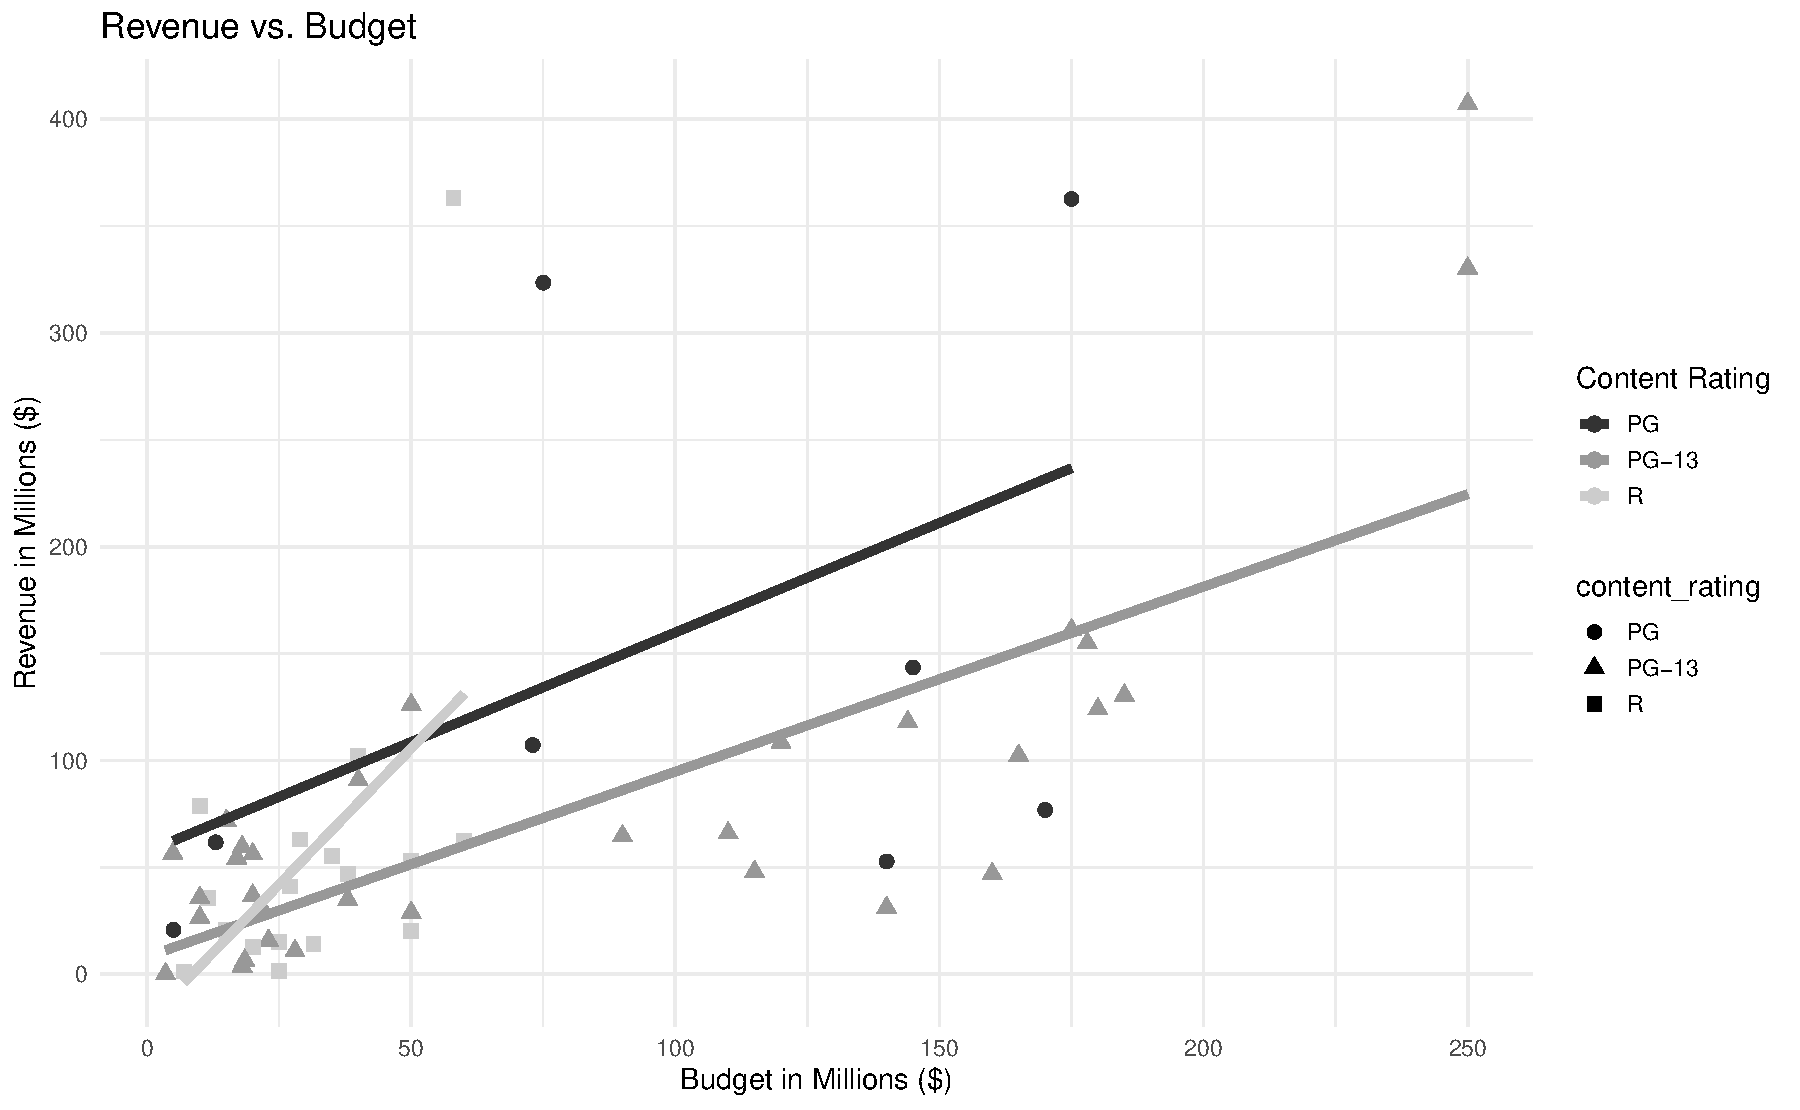
\includegraphics[width=0.6\linewidth]{04-EDA-quantitative_files/figure-latex/unnamed-chunk-5-1} \end{center}

\begin{enumerate}
\def\labelenumi{\arabic{enumi}.}
\setcounter{enumi}{11}
\tightlist
\item
  Answer the following questions about the box plots above.
\end{enumerate}

\begin{enumerate}
\def\labelenumi{\alph{enumi}.}
\item
  Which content rating has the highest center?
  \vspace{0.2in}
\item
  Which content rating has the largest spread?
  \vspace{0.2in}
\item
  Which content rating is the most symmetric distribution?
  \vspace{0.2in}
\item
  Fifty percent of movies in 2016 with a PG-13 content rating fall below what value?
  \vspace{0.2in}
\item
  What is the value for the third quartile (Q3) for the PG-13 rating? Interpret this value in context.
  \vspace{.5in}
\end{enumerate}

\hypertarget{additional-notes}{%
\section{Additional notes}\label{additional-notes}}

Use this space to summarize your thoughts and take additional notes on today's activity.

\hypertarget{movie-profits}{%
\chapter{Movie Profits}\label{movie-profits}}

\hypertarget{learning-objectives}{%
\section{Learning objectives}\label{learning-objectives}}

\begin{itemize}
\item
  Identify and create appropriate summary statistics and plots
  given a data set with two quantitative variables
\item
  Use scatterplots to assess the relationship between two quantitative variables
\item
  Find the correlation coefficient
\item
  Find the estimated line of regression using summary statistics and \texttt{R} linear model (\texttt{lm}) output
\item
  Interpret the slope coefficient in context of the problem
\item
  Interpret the coefficient of determination in context of the problem
\end{itemize}

\hypertarget{terminology-review}{%
\section{Terminology review}\label{terminology-review}}

In today's activity, we will review summary measures and plots for two quantitative variables. Some terms covered in this activity are:

\begin{itemize}
\item
  Scatterplot
\item
  Correlation
\item
  Slope
\item
  Least-squares line of regression
\item
  Coefficient of determination (\(r\)-squared)
\end{itemize}

To review these concepts, see Chapter 3 in the textbook.

\hypertarget{movies-released-in-2016}{%
\section{Movies released in 2016}\label{movies-released-in-2016}}

We will revisit the data set used last week collected on Movies released in 2016. Here is a reminder of the variables collected on these movies.

\begin{longtable}[]{@{}ll@{}}
\toprule
\begin{minipage}[b]{0.22\columnwidth}\raggedright
\textbf{Variable}\strut
\end{minipage} & \begin{minipage}[b]{0.72\columnwidth}\raggedright
\textbf{Description}\strut
\end{minipage}\tabularnewline
\midrule
\endhead
\begin{minipage}[t]{0.22\columnwidth}\raggedright
\texttt{budget\_mil}\strut
\end{minipage} & \begin{minipage}[t]{0.72\columnwidth}\raggedright
Amount of money (in US \$ millions) budgeted for the production of the movie\strut
\end{minipage}\tabularnewline
\begin{minipage}[t]{0.22\columnwidth}\raggedright
\texttt{revenue\_mil}\strut
\end{minipage} & \begin{minipage}[t]{0.72\columnwidth}\raggedright
Amount of money (in US \$ millions) the movie made after release\strut
\end{minipage}\tabularnewline
\begin{minipage}[t]{0.22\columnwidth}\raggedright
\texttt{duration}\strut
\end{minipage} & \begin{minipage}[t]{0.72\columnwidth}\raggedright
Length of the movie (in minutes)\strut
\end{minipage}\tabularnewline
\begin{minipage}[t]{0.22\columnwidth}\raggedright
\texttt{content\_rating}\strut
\end{minipage} & \begin{minipage}[t]{0.72\columnwidth}\raggedright
Rating of the movie (\texttt{G}, \texttt{PG}, \texttt{PG-13}, \texttt{R}, \texttt{Not\ Rated})\strut
\end{minipage}\tabularnewline
\begin{minipage}[t]{0.22\columnwidth}\raggedright
\texttt{imdb\_score}\strut
\end{minipage} & \begin{minipage}[t]{0.72\columnwidth}\raggedright
IMDb user rating score from 1 to 10\strut
\end{minipage}\tabularnewline
\begin{minipage}[t]{0.22\columnwidth}\raggedright
\texttt{genres}\strut
\end{minipage} & \begin{minipage}[t]{0.72\columnwidth}\raggedright
Categories the movie falls into (e.g., Action, Drama, etc.)\strut
\end{minipage}\tabularnewline
\begin{minipage}[t]{0.22\columnwidth}\raggedright
\texttt{movie\_facebook\_likes}\strut
\end{minipage} & \begin{minipage}[t]{0.72\columnwidth}\raggedright
Number of likes a movie receives on Facebook\strut
\end{minipage}\tabularnewline
\bottomrule
\end{longtable}

\newpage

\hypertarget{vocabulary-review}{%
\subsection{Vocabulary review}\label{vocabulary-review}}

\begin{enumerate}
\def\labelenumi{\arabic{enumi}.}
\tightlist
\item
  What type of plot is used to display two quantitative variables?
\end{enumerate}

\vspace{0.2in}

\begin{enumerate}
\def\labelenumi{\arabic{enumi}.}
\setcounter{enumi}{1}
\tightlist
\item
  What summary statistics are used to describe the relationship between two quantitative variables?
\end{enumerate}

\vspace{0.3in}

We will look at the relationship between `Budget' and `Revenue' for movies released in 2016. This shows a scatterplot of `Budget' as a predictor of `Revenue' (note: both variables are measures in ``millions of dollars'').

\begin{Shaded}
\begin{Highlighting}[]
\NormalTok{movies \textless{}{-}}\StringTok{ }\KeywordTok{read.csv}\NormalTok{(}\StringTok{"data/Movies2016.csv"}\NormalTok{) }\CommentTok{\#Reads in data set}
\NormalTok{movies }\OperatorTok{\%\textgreater{}\%}\StringTok{ }\CommentTok{\#Data set pipes into...}
\KeywordTok{ggplot}\NormalTok{(}\KeywordTok{aes}\NormalTok{(}\DataTypeTok{x =}\NormalTok{ budget\_mil, }\DataTypeTok{y =}\NormalTok{ revenue\_mil))}\OperatorTok{+}\StringTok{  }\CommentTok{\#Specify variables}
\StringTok{  }\KeywordTok{geom\_point}\NormalTok{() }\OperatorTok{+}\StringTok{  }\CommentTok{\#Add scatterplot of points}
\StringTok{  }\KeywordTok{labs}\NormalTok{(}\DataTypeTok{x =} \StringTok{"Budget in Millions ($)"}\NormalTok{,  }\CommentTok{\#Label x{-}axis}
       \DataTypeTok{y =} \StringTok{"Revenue in Millions ($)"}\NormalTok{,  }\CommentTok{\#Label y{-}axis}
       \DataTypeTok{title =} \StringTok{"Revenue vs. Budget"}\NormalTok{) }\OperatorTok{+}\StringTok{ }\CommentTok{\#Be sure to tile your plots}
\StringTok{  }\KeywordTok{geom\_smooth}\NormalTok{(}\DataTypeTok{method =} \StringTok{"lm"}\NormalTok{, }\DataTypeTok{se =} \OtherTok{FALSE}\NormalTok{)  }\CommentTok{\#Add regression line}
\end{Highlighting}
\end{Shaded}

\begin{center}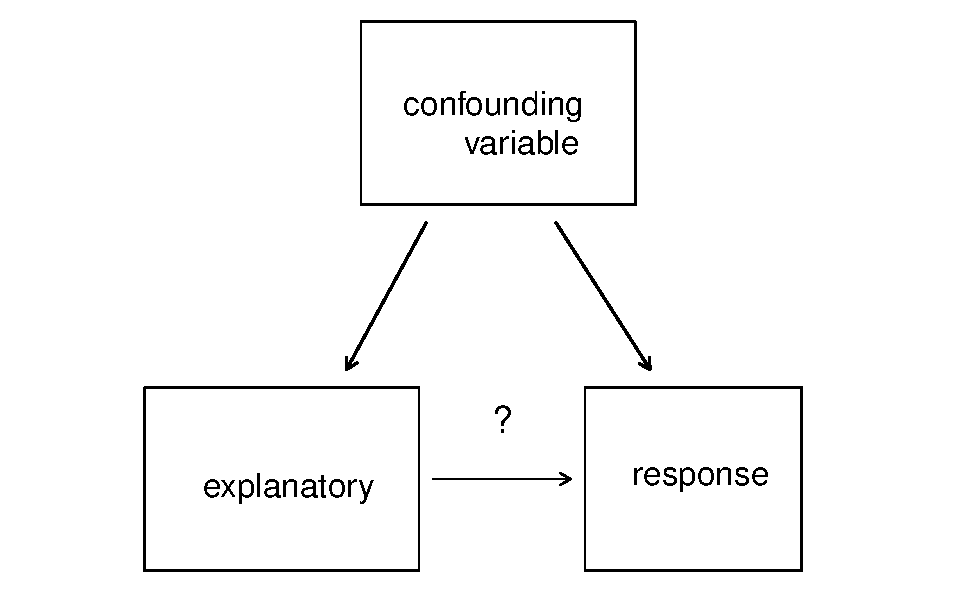
\includegraphics[width=0.7\linewidth]{05-EDA-multivariate_files/figure-latex/unnamed-chunk-1-1} \end{center}

\begin{enumerate}
\def\labelenumi{\arabic{enumi}.}
\setcounter{enumi}{2}
\tightlist
\item
  Assess the four features of the scatterplot that describe this relationship. Describe each feature using a complete sentence!
\end{enumerate}

\begin{itemize}
\tightlist
\item
  Form (linear, non-linear)
\end{itemize}

\vspace{.4in}

\begin{itemize}
\tightlist
\item
  Direction (positive, negative)
\end{itemize}

\vspace{.4in}

\begin{itemize}
\tightlist
\item
  Strength
\end{itemize}

\vspace{.4in}

\begin{itemize}
\tightlist
\item
  Unusual observations or outliers
\end{itemize}

\vspace{.4in}

\newpage

\begin{enumerate}
\def\labelenumi{\arabic{enumi}.}
\setcounter{enumi}{3}
\tightlist
\item
  Does there appear to be an association between `Budget' and `Revenue'? Explain.
\end{enumerate}

\vspace{1in}

\hypertarget{correlation}{%
\subsection{Correlation}\label{correlation}}

Correlation measures the strength and the direction between two quantitative variables. The closer the value of correlation to + or - 1 the stronger the linear relationship. Values close to zero indicate a very weak linear relationship between the two variables. The following output shows a correlation matrix between several pairs of quantitative variables.

\begin{Shaded}
\begin{Highlighting}[]
\CommentTok{\# Take subset of variables}
\NormalTok{movies }\OperatorTok{\%\textgreater{}\%}\StringTok{  }\CommentTok{\#Data set pipes into...}
\StringTok{  }\KeywordTok{select}\NormalTok{(}\KeywordTok{c}\NormalTok{(}\StringTok{"budget\_mil"}\NormalTok{, }\StringTok{"revenue\_mil"}\NormalTok{,  }\CommentTok{\# Take subset of variables}
           \StringTok{"duration"}\NormalTok{, }\StringTok{"imdb\_score"}\NormalTok{, }
           \StringTok{"movie\_facebook\_likes"}\NormalTok{)) }\OperatorTok{\%\textgreater{}\%}
\StringTok{  }\KeywordTok{cor}\NormalTok{(}\DataTypeTok{use=}\StringTok{"pairwise.complete.obs"}\NormalTok{) }\OperatorTok{\%\textgreater{}\%}\StringTok{ }\CommentTok{\# Calculate correlation matrix}
\StringTok{  }\KeywordTok{round}\NormalTok{(}\DecValTok{3}\NormalTok{)  }\CommentTok{\# Round to 3 decimals}
\end{Highlighting}
\end{Shaded}

\begin{verbatim}
#>                      budget_mil revenue_mil duration imdb_score
#> budget_mil                1.000       0.686    0.463      0.292
#> revenue_mil               0.686       1.000    0.227      0.398
#> duration                  0.463       0.227    1.000      0.261
#> imdb_score                0.292       0.398    0.261      1.000
#> movie_facebook_likes      0.678       0.723    0.438      0.309
#>                      movie_facebook_likes
#> budget_mil                          0.678
#> revenue_mil                         0.723
#> duration                            0.438
#> imdb_score                          0.309
#> movie_facebook_likes                1.000
\end{verbatim}

\begin{enumerate}
\def\labelenumi{\arabic{enumi}.}
\setcounter{enumi}{4}
\tightlist
\item
  Using the output above, which two variables have the strongest correlation?
\end{enumerate}

\vspace{0.3in}

\begin{enumerate}
\def\labelenumi{\arabic{enumi}.}
\setcounter{enumi}{5}
\tightlist
\item
  What is the value of correlation between `Budget' and `Revenue'?
\end{enumerate}

\vspace{0.3in}

\begin{enumerate}
\def\labelenumi{\arabic{enumi}.}
\setcounter{enumi}{6}
\tightlist
\item
  Based on the value of correlation what would the sign of the slope be? Positive or negative? Explain.
\end{enumerate}

\vspace{0.5in}

\begin{enumerate}
\def\labelenumi{\arabic{enumi}.}
\setcounter{enumi}{7}
\tightlist
\item
  Does your answer to question 7 match the direction you choose in question 3?
\end{enumerate}

\vspace{0.2in}

\begin{enumerate}
\def\labelenumi{\arabic{enumi}.}
\setcounter{enumi}{8}
\tightlist
\item
  Explain why the correlation values on the diagonal are equal to 1.
\end{enumerate}

\vspace{1in}

\newpage

\hypertarget{slope}{%
\subsection{Slope}\label{slope}}

The linear model function in R gives us the summary for the least squares regression line. The estimate for (Intercept) is the y-intercept for the line of least squares and the estimate for budget\_mil is the value of \(b_1\), the slope.

\begin{Shaded}
\begin{Highlighting}[]
\CommentTok{\# Fit linear model: y \textasciitilde{} x}
\NormalTok{revenueLM \textless{}{-}}\StringTok{ }\KeywordTok{lm}\NormalTok{(revenue\_mil }\OperatorTok{\textasciitilde{}}\StringTok{ }\NormalTok{budget\_mil, }\DataTypeTok{data=}\NormalTok{movies)}
\KeywordTok{summary}\NormalTok{(revenueLM)}\OperatorTok{$}\NormalTok{coefficients }\CommentTok{\# Display coefficient summary}
\end{Highlighting}
\end{Shaded}

\begin{verbatim}
#>              Estimate Std. Error  t value     Pr(>|t|)
#> (Intercept) 9.1693054  9.0175499 1.016829 3.119606e-01
#> budget_mil  0.9460001  0.1056786 8.951670 4.339561e-14
\end{verbatim}

You may remember from middle and high school that slope \(=\frac{\mbox{rise}}{\mbox{run}}\).

Using \(b_1\) to represent slope, we can write that as the fraction \(\frac{b_1}{1}\).

Therefore, the slope predicts the how much the line will \emph{rise} for each \emph{run} of +1. In other words, as the \(x\) variable increases by 1 unit, the \(y\) variable is expected to change (increase/decrease) by the value of slope.

\begin{enumerate}
\def\labelenumi{\arabic{enumi}.}
\setcounter{enumi}{9}
\tightlist
\item
  Write out the least squares line using the summary statistics provided in proper statistical notation.
\end{enumerate}

\vspace{.6in}

\begin{enumerate}
\def\labelenumi{\arabic{enumi}.}
\setcounter{enumi}{10}
\tightlist
\item
  Interpret the value of slope in context of the problem.
\end{enumerate}

\vspace{1in}

\begin{enumerate}
\def\labelenumi{\arabic{enumi}.}
\setcounter{enumi}{11}
\tightlist
\item
  Using the least squares line from question 10, predict the revenue for a movie with a budget of 165 million.
\end{enumerate}

\vspace{.6in}

\hypertarget{residuals}{%
\subsection{Residuals}\label{residuals}}

The model we are using assumes the relationship between the two variables follows a straight line. The residuals are the errors, or the part that hasn't been modeled by the line.

\begin{center}
Data = Model + Residual

Residual = Data - Model

$e_i=y_i-\hat{y}_i$
\end{center}

\begin{enumerate}
\def\labelenumi{\arabic{enumi}.}
\setcounter{enumi}{12}
\tightlist
\item
  The movie, \emph{Independence Day: Resurgence}, had a budget of 165 million and revenue of 102.315 million. Find the residual for this movie.
\end{enumerate}

\vspace{.8in}

\begin{enumerate}
\def\labelenumi{\arabic{enumi}.}
\setcounter{enumi}{13}
\tightlist
\item
  Did the line of regression overestimate or underestimate the revenue for this movie?
\end{enumerate}

\vspace{.2in}

\newpage

\hypertarget{coefficient-of-determination-squared-correlation}{%
\subsection{Coefficient of determination (squared correlation)}\label{coefficient-of-determination-squared-correlation}}

The coefficient of determination, \(r^2\), can also be used to describe the strength of the linear relationship between two quantitative variables. \(r^2\) measures the proportion of variation in the response that is explained by the least squares line with the explanatory variable.

\begin{enumerate}
\def\labelenumi{\arabic{enumi}.}
\setcounter{enumi}{14}
\tightlist
\item
  Use the correlation, \(r\), to calculate the coefficient of determination between `Budget' and `Revenue', \(r^2\).
\end{enumerate}

\vspace{.4in}

\begin{enumerate}
\def\labelenumi{\arabic{enumi}.}
\setcounter{enumi}{15}
\tightlist
\item
  Interpret the coefficient of determination in context of the problem.
\end{enumerate}

\vspace{.6in}

\hypertarget{multivariate-plots}{%
\subsection{Multivariate plots}\label{multivariate-plots}}

What if we wanted to see if the relationship between `Budget' and `Revenue' differs if we add another variable into the picture? The following plot visualized three variables, creating a \textbf{multivariate} plot.

\begin{Shaded}
\begin{Highlighting}[]
\NormalTok{movies }\OperatorTok{\%\textgreater{}\%}\StringTok{ }\CommentTok{\#Data set pipes into...}
\KeywordTok{ggplot}\NormalTok{(}\KeywordTok{aes}\NormalTok{(}\DataTypeTok{x =}\NormalTok{ budget\_mil, }\DataTypeTok{y =}\NormalTok{ revenue\_mil, }\DataTypeTok{color =}\NormalTok{ content\_rating)) }\OperatorTok{+}\StringTok{  }\CommentTok{\#Specify variables}
\StringTok{  }\KeywordTok{geom\_point}\NormalTok{(}\KeywordTok{aes}\NormalTok{(}\DataTypeTok{shape =}\NormalTok{ content\_rating), }\DataTypeTok{size =} \DecValTok{3}\NormalTok{) }\OperatorTok{+}\StringTok{  }\CommentTok{\#Add scatterplot of points}
\StringTok{  }\KeywordTok{labs}\NormalTok{(}\DataTypeTok{x =} \StringTok{"Budget in Millions ($)"}\NormalTok{,  }\CommentTok{\#Label x{-}axis}
       \DataTypeTok{y =} \StringTok{"Revenue in Millions ($)"}\NormalTok{,  }\CommentTok{\#Label y{-}axis}
       \DataTypeTok{color =} \StringTok{"Content Rating"}\NormalTok{,  }\CommentTok{\#Label legend}
       \DataTypeTok{title =} \StringTok{"Revenue vs. Budget"}\NormalTok{) }\OperatorTok{+}\StringTok{ }\CommentTok{\#Be sure to tile your plots}
\StringTok{  }\KeywordTok{geom\_smooth}\NormalTok{(}\DataTypeTok{method =} \StringTok{"lm"}\NormalTok{, }\DataTypeTok{se =} \OtherTok{FALSE}\NormalTok{, }\DataTypeTok{lwd =} \DecValTok{2}\NormalTok{) }\OperatorTok{+}\StringTok{ }\CommentTok{\#Add regression lines}
\StringTok{  }\KeywordTok{scale\_color\_grey}\NormalTok{() }\CommentTok{\#Make black and white}
\end{Highlighting}
\end{Shaded}

\begin{center}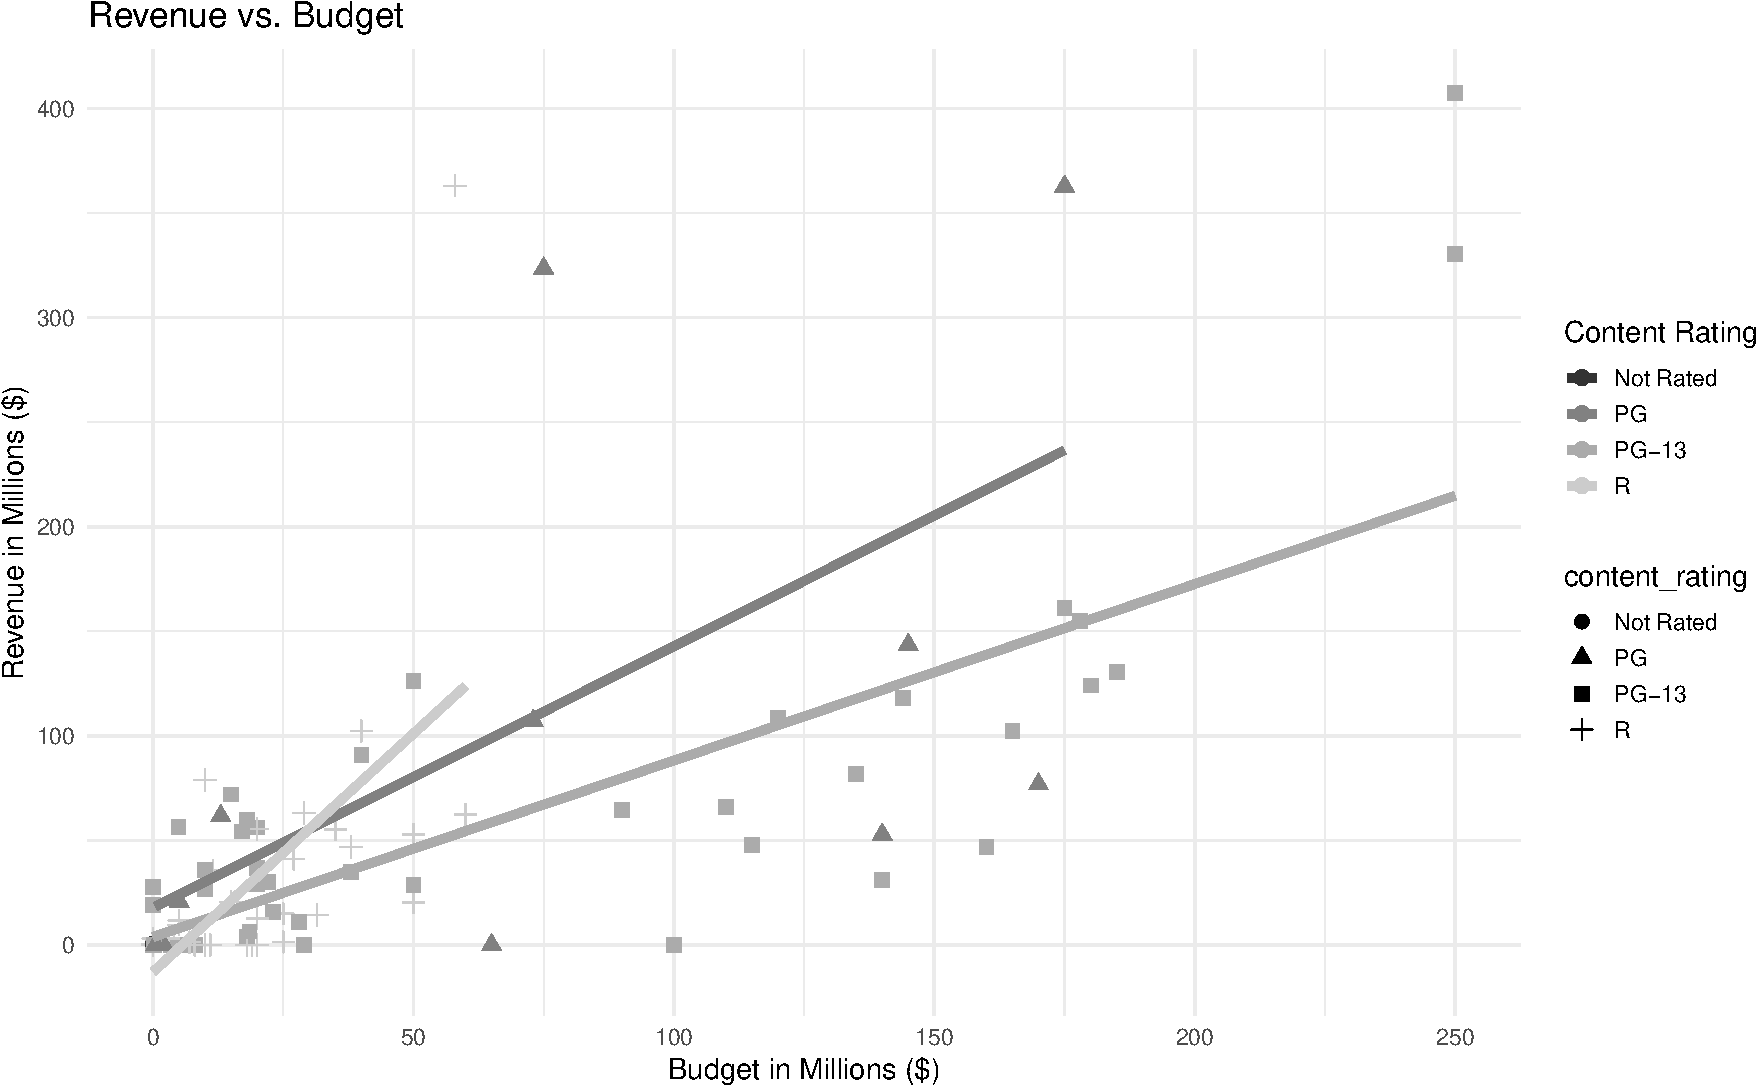
\includegraphics[width=0.7\linewidth]{05-EDA-multivariate_files/figure-latex/unnamed-chunk-4-1} \end{center}

\begin{enumerate}
\def\labelenumi{\arabic{enumi}.}
\setcounter{enumi}{24}
\tightlist
\item
  Identify the three varables plotted in this graph.
\end{enumerate}

\vspace{0.5in}

\begin{enumerate}
\def\labelenumi{\arabic{enumi}.}
\setcounter{enumi}{25}
\tightlist
\item
  Does the relationship between `Budget' and `Revenue' differ among the different content ratings? Explain.
\end{enumerate}

\vspace{1in}

\newpage

\hypertarget{additional-notes}{%
\section{Additional notes}\label{additional-notes}}

Use this space to summarize your thoughts and take additional notes on today's activity.

\hypertarget{handedness-of-male-boxers}{%
\chapter{Handedness of Male Boxers}\label{handedness-of-male-boxers}}

\hypertarget{learning-objectives}{%
\section{Learning objectives}\label{learning-objectives}}

\begin{itemize}
\item
  Identify the two possible explanations (one assuming the null hypothesis, and one assuming the alternative hypothesis) for a relationship seen in sample data
\item
  Given a research question, construct the null and alternative hypotheses
  in words and using appropriate statistical symbols
\item
  Describe and perform simulation-based hypothesis tests for a single proportion
\item
  Interpret and evaluate a p-value
\item
  Use bootstrapping to find a confidence interval for a single proportion
\item
  Interpret a confidence interval
\end{itemize}

\hypertarget{terminology-review}{%
\section{Terminology review}\label{terminology-review}}

In today's activity, we will introduce simulation hypothesis testing and confidence intervals for a single categorical variable. Some terms covered in this activity are:

\begin{itemize}
\item
  Parameter of interest
\item
  Null hypothesis
\item
  Alternative hypothesis
\item
  Simulation
\item
  Null distribution
\item
  p-value
\item
  Bootstrapping
\item
  Confidence interval
\end{itemize}

To review these concepts, see Chapter 5 in your textbook, focusing on Sections 5.1 through 5.3.

\hypertarget{steps-of-the-statistical-investigation-process}{%
\section{Steps of the statistical investigation process}\label{steps-of-the-statistical-investigation-process}}

We will work through a six-step process to complete a hypothesis test for a single proportion.

\begin{itemize}
\item
  \textbf{Ask a research question} that can be addressed by collecting data. What are the researchers trying to show?
\item
  \textbf{Design a study and collect data}. This step involves selecting the people or objects to be studied and how to gather relevant data on them.
\item
  \textbf{Summarize and visualize the data}. Calculate summary statistics and create graphical plots that best represent the research question.
\item
  \textbf{Use statistical analysis methods to draw inferences from the data}. Choose an analysis technique appropriate for the data and identify the p-value. In this study, we will focus on using randomization.
\item
  \textbf{Communicate the results and answer the research question}. Using the p-value and confidence interval from the analysis, determine whether the data provide statistical evidence against the null hypothesis.
\item
  \textbf{Revisit and look forward} to point out limitations of the study and suggest new studies that could be performed to build on the findings of the study
\end{itemize}

\hypertarget{handedness-of-male-boxers-1}{%
\section{Handedness of male boxers}\label{handedness-of-male-boxers-1}}

Left-handedness is a trait that is found in about 10\% of the population. Past studies have shown that left-handed men are over-represented among professional fighters. The fighting claim states that left-handed men have an advantage in competition. In this random sample of 500 male boxers we will see if there is an over-prevalence of left-handed fighters.

\begin{Shaded}
\begin{Highlighting}[]
\NormalTok{handedness \textless{}{-}}\StringTok{ }\KeywordTok{read.csv}\NormalTok{(}\StringTok{"data/Male\_boxers.csv"}\NormalTok{) }\CommentTok{\# Read in data set}
\KeywordTok{set.seed}\NormalTok{(}\DecValTok{12980}\NormalTok{) }\CommentTok{\# Set random number generator to select }
                \CommentTok{\# same sample each time.}
                \CommentTok{\# Remove this line to get a different random sample.}
\NormalTok{handedness\_sub \textless{}{-}}\StringTok{ }\NormalTok{handedness }\OperatorTok{\%\textgreater{}\%}
\StringTok{  }\KeywordTok{select}\NormalTok{(Stance) }\OperatorTok{\%\textgreater{}\%}\StringTok{ }\CommentTok{\# Select Stance variable}
\StringTok{  }\KeywordTok{sample\_n}\NormalTok{(}\DecValTok{500}\NormalTok{, }\DataTypeTok{replace=}\OtherTok{FALSE}\NormalTok{) }\CommentTok{\# Randomly sample 500 rows}
\KeywordTok{dim}\NormalTok{(handedness\_sub) }\CommentTok{\# Check dimensions of data set are 500 rows x 1 col}
\end{Highlighting}
\end{Shaded}

\begin{verbatim}
#> [1] 500   1
\end{verbatim}

\hypertarget{summary-statistics-review}{%
\subsection{Summary statistics review}\label{summary-statistics-review}}

\begin{enumerate}
\def\labelenumi{\arabic{enumi}.}
\tightlist
\item
  What are the observational units?
\end{enumerate}

\vspace{0.5in}

\begin{enumerate}
\def\labelenumi{\arabic{enumi}.}
\setcounter{enumi}{1}
\tightlist
\item
  What variable are we testing? Is it categorical or quantitative?
\end{enumerate}

\vspace{0.5in}

\begin{enumerate}
\def\labelenumi{\arabic{enumi}.}
\setcounter{enumi}{2}
\tightlist
\item
  What type of plot would be appropriate to visually display the data?
\end{enumerate}

\vspace{0.5in}

\begin{enumerate}
\def\labelenumi{\arabic{enumi}.}
\setcounter{enumi}{3}
\tightlist
\item
  Write out in context the statistic will we calculate to summarize the data.
\end{enumerate}

\vspace{0.5in}

\hypertarget{ask-a-research-question}{%
\subsection{Ask a research question}\label{ask-a-research-question}}

\begin{enumerate}
\def\labelenumi{\arabic{enumi}.}
\setcounter{enumi}{4}
\tightlist
\item
  Identify the research question for this study.
\end{enumerate}

\vspace{1in}

\hypertarget{design-a-study-and-collect-data}{%
\subsection{Design a study and collect data}\label{design-a-study-and-collect-data}}

\begin{enumerate}
\def\labelenumi{\arabic{enumi}.}
\setcounter{enumi}{5}
\tightlist
\item
  What is the target population for this study?
\end{enumerate}

\vspace{0.5in}

\begin{enumerate}
\def\labelenumi{\arabic{enumi}.}
\setcounter{enumi}{6}
\tightlist
\item
  Did the researchers use a biased or an unbiased method of selection? Explain your answer.
\end{enumerate}

\vspace{1in}

\hypertarget{summarize-and-visualize-the-data}{%
\subsection{Summarize and visualize the data}\label{summarize-and-visualize-the-data}}

\begin{Shaded}
\begin{Highlighting}[]
\NormalTok{handedness\_sub }\OperatorTok{\%\textgreater{}\%}\StringTok{ }\KeywordTok{count}\NormalTok{(Stance)  }\CommentTok{\# Count number in each Stance category}
\end{Highlighting}
\end{Shaded}

\begin{verbatim}
#> Warning: `count_()` is deprecated as of dplyr 0.7.0.
#> Please use `count()` instead.
#> See vignette('programming') for more help
#> This warning is displayed once every 8 hours.
#> Call `lifecycle::last_warnings()` to see where this warning was generated.
\end{verbatim}

\begin{verbatim}
#>         Stance   n
#> 1  left-handed  81
#> 2 right-handed 419
\end{verbatim}

\begin{enumerate}
\def\labelenumi{\arabic{enumi}.}
\setcounter{enumi}{7}
\tightlist
\item
  Calculate the appropriate summary statistic that represents the research question. Use appropriate notation.
\end{enumerate}

\vspace{0.5in}

\hypertarget{use-statistical-analysis-methods-to-draw-inferences-from-the-data}{%
\subsection{Use statistical analysis methods to draw inferences from the data}\label{use-statistical-analysis-methods-to-draw-inferences-from-the-data}}

When testing data we must first identify the null hypothesis. The null hypothesis is written about the parameter of interest, or the true value of interest.

\begin{enumerate}
\def\labelenumi{\arabic{enumi}.}
\setcounter{enumi}{8}
\tightlist
\item
  Write out the parameter of interest for this study. (Hint: the true proportion of\ldots.)
\end{enumerate}

\vspace{1in}

\begin{enumerate}
\def\labelenumi{\arabic{enumi}.}
\setcounter{enumi}{9}
\tightlist
\item
  Using the parameter of interest in question 9, write out the null hypothesis in words.
\end{enumerate}

\vspace{1in}

\newpage

The notation used for a true proportion is \(\pi\). Since this summarizes a population, it is a parameter. When writing the \textbf{null hypothesis} in notation we set the parameter equal to the null value, \(H_0: \pi = \pi_0\)

\begin{enumerate}
\def\labelenumi{\arabic{enumi}.}
\setcounter{enumi}{10}
\tightlist
\item
  Write the null hypothesis in notation using the null value of 0.1 in place of \(\pi_0\).
\end{enumerate}

\vspace{0.5in}

The \textbf{alternative hypothesis} is the claim to be tested and the direction is based on the research question.

\begin{enumerate}
\def\labelenumi{\arabic{enumi}.}
\setcounter{enumi}{11}
\tightlist
\item
  Based on the research question from question 5, are we testing that the parameter is greater than 0.1, less than 0.1 or different than 0.1?
\end{enumerate}

\vspace{0.5in}

\begin{enumerate}
\def\labelenumi{\arabic{enumi}.}
\setcounter{enumi}{12}
\tightlist
\item
  Write out the alternative hypothesis in words.
\end{enumerate}

\vspace{1in}

\begin{enumerate}
\def\labelenumi{\arabic{enumi}.}
\setcounter{enumi}{13}
\tightlist
\item
  Write out the alternative hypothesis in notation.
\end{enumerate}

\vspace{0.5in}

Remember that when utilizing a hypothesis test, we are evaluating two competing possibilities. For this study the \textbf{two possibilities} are either\ldots{}

\begin{itemize}
\item
  The true proportion of male boxers who are left handed is 0.1 and our results just occurred by random chance or
\item
  The true proportion of male boxers who are left handed is greater than 0.1 and our results reflect this
\end{itemize}

Notice that these two competing possibilities represent the null and alternative hypotheses.

The null distribution is created under the assumption the null hypothesis is true. In this case, we assume the true proportion of male boxers who are left handed is 0.1 so we will create 1000 different simulations of 500 boxers under this assumption.

Let's think about how to use cards to create one simulation of 500 boxers under the assumption the null hypothesis is true. Suppose blue cards represents left-handed and red cards represents right-handed.

\begin{enumerate}
\def\labelenumi{\arabic{enumi}.}
\setcounter{enumi}{14}
\tightlist
\item
  How many cards total do we need? How many blue ones? How many red ones?
\end{enumerate}

\vspace{0.5in}

\begin{enumerate}
\def\labelenumi{\arabic{enumi}.}
\setcounter{enumi}{15}
\tightlist
\item
  Next, we would mix the cards together and draw 1 card, write down if it's red or blue, and replace the card. How many times would we need to repeat this process to simulate our sample?
\end{enumerate}

\vspace{0.5in}

\begin{enumerate}
\def\labelenumi{\arabic{enumi}.}
\setcounter{enumi}{16}
\tightlist
\item
  Once we have one simulated sample, what would we calculate and plot on the null distribution?
  \vspace{1in}
\end{enumerate}

We will use the computer to simulate a null distribution of 1000 different samples of 500 male boxers, plotting the proportion who are left handed in each sample, based on the assumption that the true proportion of male boxers who are left handed is 0.1 (or that the null hypothesis is true).

To use the computer simulation, we will need to enter the ``probability of success'' (\(\pi_0\)), ``sample size'' (the number of observational units in the sample), ``number of repetitions'' (the number of samples to be generated), ``as extreme as'' (the observed statistic), and the ``direction'' (matches the direction of the alternative hypothesis).

\begin{enumerate}
\def\labelenumi{\arabic{enumi}.}
\setcounter{enumi}{17}
\tightlist
\item
  What values should be entered into the simulation?
\end{enumerate}

\vspace{.2in}

\begin{itemize}
\tightlist
\item
  Probability of success:
\end{itemize}

\vspace{.2in}

\begin{itemize}
\tightlist
\item
  Sample size:
\end{itemize}

\vspace{.2in}

\begin{itemize}
\tightlist
\item
  Number of repetitions:
\end{itemize}

\vspace{.2in}

\begin{itemize}
\tightlist
\item
  As extreme as:
\end{itemize}

\vspace{.2in}

\begin{itemize}
\tightlist
\item
  Direction:
\end{itemize}

\newpage

The following \texttt{R} code produced the null distribution with 1000 simulations that follows. Check that your answers to question 18 match the code inputs.

\begin{Shaded}
\begin{Highlighting}[]
\KeywordTok{one\_proportion\_test}\NormalTok{(}\DataTypeTok{probability\_success =} \FloatTok{0.1}\NormalTok{, }\CommentTok{\#Null hypothesis value}
                    \DataTypeTok{sample\_size =} \DecValTok{500}\NormalTok{, }\CommentTok{\#Enter sample size}
                    \DataTypeTok{number\_repetitions =} \DecValTok{1000}\NormalTok{, }\CommentTok{\#Enter number of simulations}
                    \DataTypeTok{as\_extreme\_as =} \DecValTok{81}\OperatorTok{/}\DecValTok{500}\NormalTok{, }\CommentTok{\#observed statistic}
                    \DataTypeTok{direction =} \StringTok{"greater"}\NormalTok{, }\CommentTok{\#specify direction of alternative hypothesis}
                    \DataTypeTok{report\_value =} \StringTok{"proportion"}\NormalTok{) }\CommentTok{\#Reporting proportion or number of successes?}
\end{Highlighting}
\end{Shaded}

\begin{center}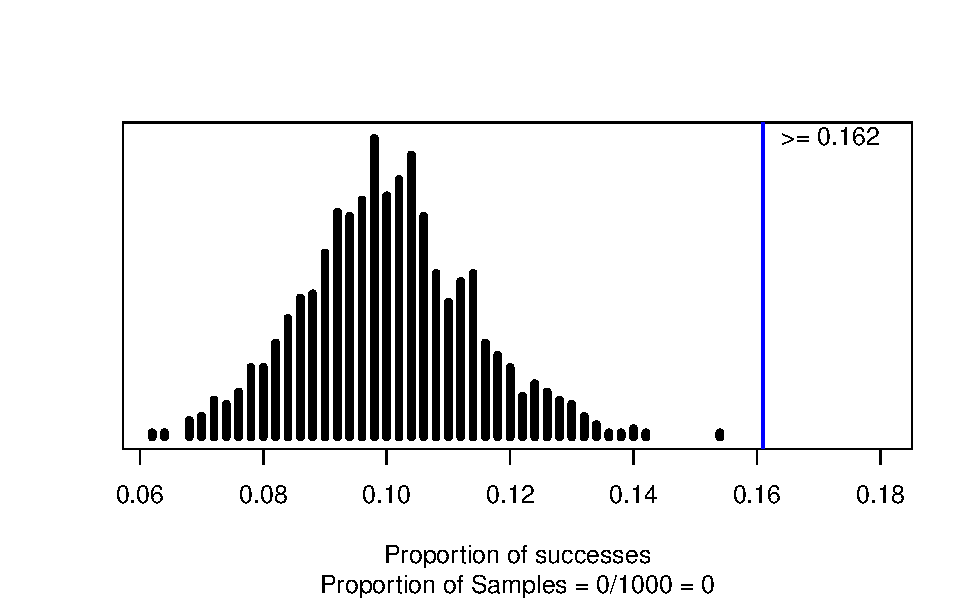
\includegraphics[width=0.7\linewidth]{06-inference-1cat_files/figure-latex/unnamed-chunk-4-1} \end{center}

\begin{enumerate}
\def\labelenumi{\arabic{enumi}.}
\setcounter{enumi}{18}
\tightlist
\item
  Around what value is the null distribution centered? Why does that make sense?
\end{enumerate}

\vspace{1in}

\begin{enumerate}
\def\labelenumi{\arabic{enumi}.}
\setcounter{enumi}{19}
\tightlist
\item
  Where does the statistic (value from question 8) fall in the null distribution? Is it towards the center or in one of the tails?
\end{enumerate}

\vspace{1in}

\begin{enumerate}
\def\labelenumi{\arabic{enumi}.}
\setcounter{enumi}{20}
\tightlist
\item
  Is the statistic likely to happen or unlikely to happen if the true proportion of male boxers is 0.1? Explain your answer.
\end{enumerate}

\vspace{1in}

\begin{enumerate}
\def\labelenumi{\arabic{enumi}.}
\setcounter{enumi}{21}
\tightlist
\item
  Using the simulation, what is the proportion of samples at this summary statistic or greater, if the true proportion of male boxers is 0.1? \emph{Hint: Look under the simulation.}
\end{enumerate}

\vspace{1in}

~~~~~~~~This is the \textbf{p-value}. The smaller the p-value the more evidence we have against the null hypothesis.

\begin{enumerate}
\def\labelenumi{\arabic{enumi}.}
\setcounter{enumi}{22}
\tightlist
\item
  Using the following guidelines for the strength of evidence, how much evidence do the data provide against the null hypothesis? (Circle one.)
\end{enumerate}

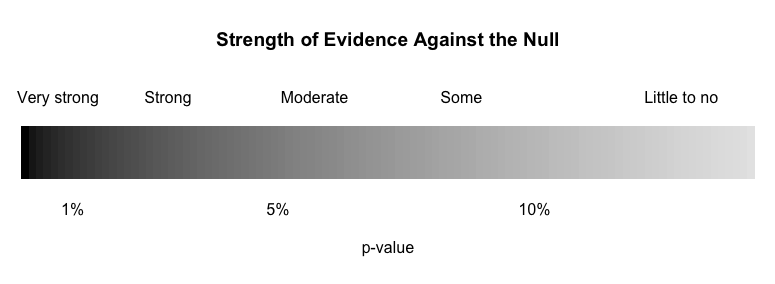
\includegraphics{images/soe_gradient_grayscale.png}

A \textbf{point estimate} provides a single plausible value for a parameter. However, a point estimate is rarely perfect; usually there is some error in the estimate. In addition to supplying a point estimate of a parameter, a next logical step would be to provide a plausible range of values for the parameter. This plausible range of values for the population parameter is called a confidence interval.

We will use bootstrapping to find the 95\% confidence interval.

\begin{enumerate}
\def\labelenumi{\arabic{enumi}.}
\setcounter{enumi}{23}
\tightlist
\item
  In your own words, explain the bootstrapping process.
  \vspace{1in}
\end{enumerate}

The following \texttt{R} code produced the following bootstrap distribution with 1000 simulations.

\begin{Shaded}
\begin{Highlighting}[]
\KeywordTok{one\_proportion\_bootstrap\_CI}\NormalTok{(}\DataTypeTok{sample\_size =} \DecValTok{500}\NormalTok{, }\CommentTok{\#Sample size}
                    \DataTypeTok{number\_successes =} \DecValTok{81}\NormalTok{, }\CommentTok{\#Observed number of successes}
                    \DataTypeTok{number\_repetitions =} \DecValTok{1000}\NormalTok{, }\CommentTok{\#Number of bootstrap samples to use}
                    \DataTypeTok{confidence\_level =} \FloatTok{0.95}\NormalTok{) }\CommentTok{\#Confidence level as a decimal}
\end{Highlighting}
\end{Shaded}

\begin{center}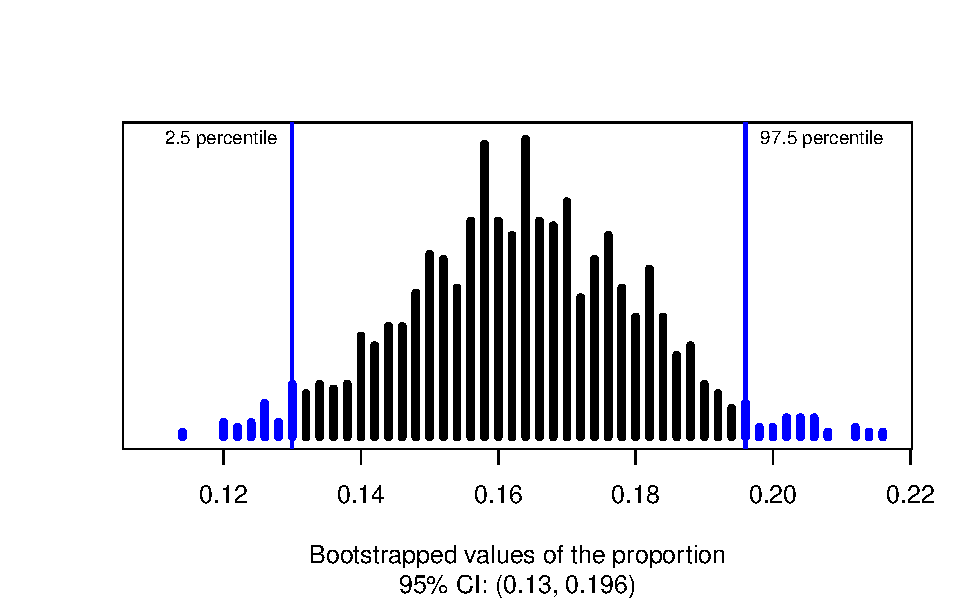
\includegraphics[width=0.7\linewidth]{06-inference-1cat_files/figure-latex/unnamed-chunk-6-1} \end{center}

\begin{enumerate}
\def\labelenumi{\arabic{enumi}.}
\setcounter{enumi}{24}
\item
  What is the value at the center of this distribution? Why does this make sense?
  \vspace{1in}
\item
  Explain why the two vertical lines are at the 2.5th percentile and the 97.5th percentile.
\end{enumerate}

\vspace{1in}

\begin{enumerate}
\def\labelenumi{\arabic{enumi}.}
\setcounter{enumi}{26}
\tightlist
\item
  Report the 95\% bootstrapped confidence interval for \(\pi\). Use interval notation: (lower value, upper value).
\end{enumerate}

\vspace{1in}

\begin{enumerate}
\def\labelenumi{\arabic{enumi}.}
\setcounter{enumi}{27}
\tightlist
\item
  Interpret the 95\% confidence interval in context.
\end{enumerate}

\vspace{1in}

\hypertarget{communicate-the-results-and-answer-the-research-question}{%
\subsection{Communicate the results and answer the research question}\label{communicate-the-results-and-answer-the-research-question}}

When we write a conclusion we answer the research question by stating how much evidence there is for the alternative hypothesis.

\begin{enumerate}
\def\labelenumi{\arabic{enumi}.}
\setcounter{enumi}{28}
\tightlist
\item
  Write a paragraph summarizing the results. Be sure to include:
\end{enumerate}

\begin{itemize}
\item
  Summary statistic
\item
  P-value and interpretation
\item
  Conclusion (written to answer the research question)
\item
  Confidence interval and interpretation
\item
  Generalization - to what group do the results apply?
\end{itemize}

\vspace{3in}

\hypertarget{revisit-and-look-forward}{%
\subsection{Revisit and look forward}\label{revisit-and-look-forward}}

\begin{enumerate}
\def\labelenumi{\arabic{enumi}.}
\setcounter{enumi}{29}
\tightlist
\item
  Suggest a new research question that you might investigate, building on what you learned in this study.
\end{enumerate}

\vspace{1in}

\hypertarget{additional-notes}{%
\section{Additional notes}\label{additional-notes}}

Use this space to summarize your thoughts and take additional notes on today's activity.

\hypertarget{winter-sports-helmet-use-and-head-injuries}{%
\chapter{Winter Sports Helmet Use and Head Injuries}\label{winter-sports-helmet-use-and-head-injuries}}

\hypertarget{learning-objectives}{%
\section{Learning objectives}\label{learning-objectives}}

\begin{itemize}
\item
  Write out the null and alternative hypothesis for two categorical variables
\item
  Assess the conditions to use the standard normal distribution for a difference in proportions
\item
  Calculate the Z test statistic for the difference in proportions
\item
  Find the p-value and assess the strength of evidence
\item
  Create and interpret a confidence interval for the difference in proportions
\end{itemize}

\hypertarget{terminology-review}{%
\section{Terminology review}\label{terminology-review}}

In today's activity, we will use theory-based methods to analyze two categorical variables. Some terms covered in this activity are:

\begin{itemize}
\item
  Conditional proportion
\item
  Z test
\item
  \(z*\) multiplier
\item
  Null hypothesis
\item
  Alternative hypothesis
\item
  Test statistic
\item
  Standard normal distribution
\item
  Independence and Success-Failure conditions
\item
  Type 1 and Type 2 errors
\item
  Decisions
\end{itemize}

To review these concepts, see Chapter 5 in your textbook.

\newpage

\hypertarget{helmet-use-and-head-injuries}{%
\section{Helmet Use and Head Injuries}\label{helmet-use-and-head-injuries}}

In ``Helmet Use and Risk of Head Injuries in Alpine Skiers and Snowboarders'' by Sullheim et. al., in the Journal of the American Medical Association, Vol. 295, No.~8, we can see the results from a random sample 3562 skiers and snowboarders involved in accidents.

\begin{longtable}[]{@{}cccc@{}}
\toprule
& Helmet Use & No Helmet Use & Total\tabularnewline
\midrule
\endhead
Head Injury & 96 & 480 & 576\tabularnewline
No Head Injury & 656 & 2330 & 2986\tabularnewline
Total & 752 & 2810 & 3562\tabularnewline
\bottomrule
\end{longtable}

Is there evidence that safety helmet use reduces the risk of head injury for skiers and snowboarders?

\hypertarget{vocabulary-review}{%
\subsection{Vocabulary review}\label{vocabulary-review}}

\begin{enumerate}
\def\labelenumi{\arabic{enumi}.}
\tightlist
\item
  What is the explanatory variable?
\end{enumerate}

\vspace{0.5in}

\begin{enumerate}
\def\labelenumi{\arabic{enumi}.}
\setcounter{enumi}{1}
\tightlist
\item
  What is the response variable?
\end{enumerate}

\vspace{0.5in}

\begin{enumerate}
\def\labelenumi{\arabic{enumi}.}
\setcounter{enumi}{2}
\tightlist
\item
  Is this an experiment or observational study? Justify your answer.
\end{enumerate}

\vspace{0.3in}

\begin{enumerate}
\def\labelenumi{\arabic{enumi}.}
\setcounter{enumi}{3}
\tightlist
\item
  Put an X in the box that represents the appropriate scope of inference for this study.
\end{enumerate}

\begin{longtable}[]{@{}cccl@{}}
\toprule
& & Study Type &\tabularnewline
\midrule
\endhead
& & Randomized Experiment & Observational Study\tabularnewline
Selection of Cases & Random Sample & &\tabularnewline
& No Random Sample & &\tabularnewline
\bottomrule
\end{longtable}

\begin{enumerate}
\def\labelenumi{\arabic{enumi}.}
\setcounter{enumi}{4}
\tightlist
\item
  What is the conditional proportion of skiers/snowboarders with a head injury that wore a helmet?
\end{enumerate}

\vspace{.6in}

\begin{enumerate}
\def\labelenumi{\arabic{enumi}.}
\setcounter{enumi}{5}
\tightlist
\item
  What is the conditional proportion of skiers/snowboarders with a head injury that did not wear a helmet?
\end{enumerate}

\vspace{.6in}

\hypertarget{ask-a-research-question}{%
\subsection{Ask a research question}\label{ask-a-research-question}}

In this study we are looking at the relationship between two groups or two parameters (\(\pi_1\) and \(\pi_2\)). Remember we define the parameter for a categorical variable as the true proportion of observational units that are labeled as a ``success'' in the response variable.

\begin{enumerate}
\def\labelenumi{\arabic{enumi}.}
\setcounter{enumi}{6}
\tightlist
\item
  What is the variable of interest in this study?
\end{enumerate}

\vspace{0.5in}

\begin{enumerate}
\def\labelenumi{\arabic{enumi}.}
\setcounter{enumi}{7}
\item
  Write the two parameters of interest for this study. Let 1 = skier/snowboarder wore helmet, 2 = skier/snowboarder did not wear helmet.

  \(\pi_1\) -
  \vspace{0.5in}

  \(\pi_2\) -
  \vspace{0.5in}
\end{enumerate}

When comparing two groups, we assume the two parameters are equal in the null hypothesis---there is no association between the variables.

\begin{enumerate}
\def\labelenumi{\arabic{enumi}.}
\setcounter{enumi}{8}
\tightlist
\item
  Write the null hypothesis out in words using your answers to question 8.
\end{enumerate}

\vspace{1in}

\begin{enumerate}
\def\labelenumi{\arabic{enumi}.}
\setcounter{enumi}{9}
\tightlist
\item
  What is the research question?
\end{enumerate}

\vspace{1in}

\begin{enumerate}
\def\labelenumi{\arabic{enumi}.}
\setcounter{enumi}{10}
\tightlist
\item
  Based on the research question fill in the appropriate sign for the alternative hypothesis:
  \vspace{0.25in}
\end{enumerate}

~~~~~~~~~~\(H_A: \pi_1 -\pi_2\) \_\_\_\_\_\_\_\_\_\_ 0

\hypertarget{summarize-and-visualize-the-data}{%
\subsection{Summarize and visualize the data}\label{summarize-and-visualize-the-data}}

\begin{center}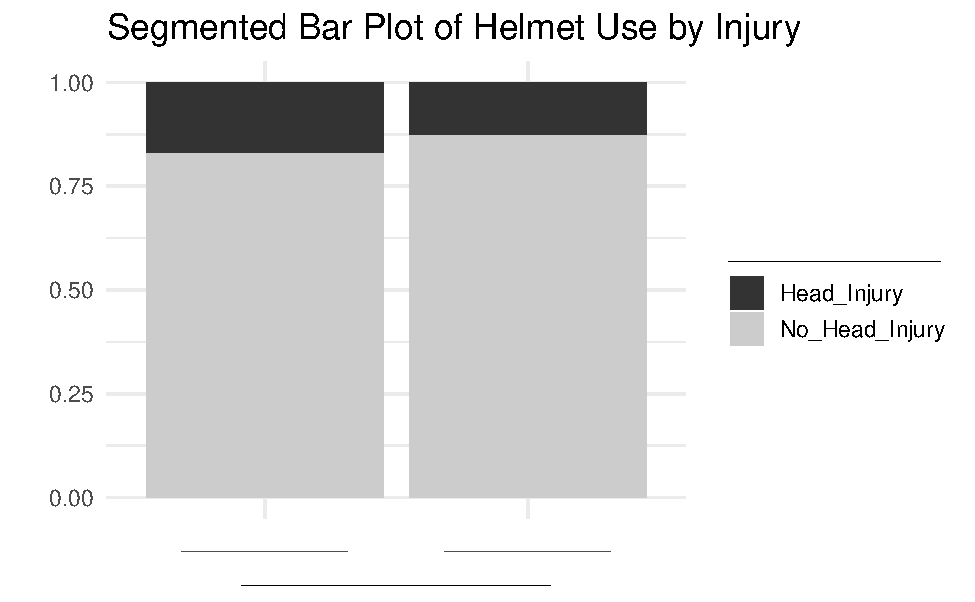
\includegraphics[width=0.7\linewidth]{07-inference-2cat_files/figure-latex/unnamed-chunk-2-1} \end{center}

\begin{enumerate}
\def\labelenumi{\arabic{enumi}.}
\setcounter{enumi}{11}
\tightlist
\item
  Fill in the blanks on the graph with the appropriate variables and values to complete the segmented bar plot showing the proportion of head injuries between those who use helmets and those who do not use helmets. *Hint: use the conditional proportions from questions 5 and 6.
\end{enumerate}

\vspace{0.1in}

\begin{enumerate}
\def\labelenumi{\arabic{enumi}.}
\setcounter{enumi}{12}
\tightlist
\item
  Based on the segmented bar plot, Does there appear to be an association between helmet use and head injury? Explain.
\end{enumerate}

\vspace{1in}

\begin{enumerate}
\def\labelenumi{\arabic{enumi}.}
\setcounter{enumi}{13}
\tightlist
\item
  Calculate the point estimate for this study. Use helmet use minus no helmet use as the order of subtraction.
\end{enumerate}

\vspace{1in}

\begin{enumerate}
\def\labelenumi{\arabic{enumi}.}
\setcounter{enumi}{14}
\tightlist
\item
  What is the notation used for the value calculated in question 14?
\end{enumerate}

\vspace{0.5in}

\hypertarget{use-statistical-analysis-methods-to-draw-inferences-from-the-data}{%
\subsection{Use statistical analysis methods to draw inferences from the data}\label{use-statistical-analysis-methods-to-draw-inferences-from-the-data}}

To test the null hypothesis we could use simulation methods as we did with a single categorical variable. In this activity we will focus on theory-based methods. Like with a single proportion, the difference in proportions can be mathematically modeled using the normal distribution if certain conditions are met.

Conditions for the sample distribution of \(\hat{p}_1-\hat{p}_2\):

\begin{itemize}
\item
  Independence: The data are independent within and between the two groups.
\item
  Success-Failure Condition: The success-failure condition holds for each group.
\end{itemize}

\vspace{.25in}

\begin{enumerate}
\def\labelenumi{\arabic{enumi}.}
\setcounter{enumi}{15}
\tightlist
\item
  Is the independence condition met? Explain your answer.
\end{enumerate}

\vspace{1in}

\begin{enumerate}
\def\labelenumi{\arabic{enumi}.}
\setcounter{enumi}{16}
\tightlist
\item
  Is the success-failure condition met for each group? Explain your answer.
\end{enumerate}

\vspace{1in}

To calculate the test statistic we use:

\begin{center}
    $Z = \frac{\text{point estimate} - \text{null value}}{SE}$

where the standard error is calculated using the pooled proportion of successes.

   $SE(\hat{p}_1-\hat{p}_2)=\sqrt{\hat{p}_{pool}(1-\hat{p}_{pool})(\frac{1}{n_1}+\frac{1}{n_2})}, \text{where}$ 
    
   $\hat{p}_{pool} = \frac{\text{number of "successes"}}{\text{number of cases}} = \frac{\hat{p}_1 n_1+\hat{p}_2 n_2}{n_1+n_2}$
    
\end{center}

\vspace{.25in}

\begin{enumerate}
\def\labelenumi{\arabic{enumi}.}
\setcounter{enumi}{17}
\tightlist
\item
  Calculate the \(SE(\hat{p}_1-\hat{p}_2)\).
\end{enumerate}

\vspace{1in}

\begin{enumerate}
\def\labelenumi{\arabic{enumi}.}
\setcounter{enumi}{18}
\tightlist
\item
  Calculate the test statistic.
\end{enumerate}

\vspace{1in}

We will use the pnorm function in \texttt{R} to find the p-value. Use the provided R markdown file and enter the value of the test statistic at xx.

\begin{Shaded}
\begin{Highlighting}[]
    \KeywordTok{pnorm}\NormalTok{(xx }\CommentTok{\#enter value of test statistic}
\NormalTok{      , }\DataTypeTok{m=}\DecValTok{0}\NormalTok{, }\DataTypeTok{s=}\DecValTok{1} \CommentTok{\#using the standard normal mean = 0, sd = 1}
\NormalTok{      , }\DataTypeTok{lower.tail=}\OtherTok{TRUE}\NormalTok{) }\CommentTok{\# gives a p{-}value less than the test statistic}
\end{Highlighting}
\end{Shaded}

\begin{enumerate}
\def\labelenumi{\arabic{enumi}.}
\setcounter{enumi}{19}
\item
  Report the p-value.
  \vspace{0.2in}
\item
  How much evidence does the p-value provide against the null hypothesis?
\end{enumerate}

\vspace{0.4in}

To find a confidence interval for the difference in proportions we will add and subtract the margin of error from the point estimate to find the two endpoints.

\[\hat{p}_1-\hat{p}_2\pm z^*SE(\hat{p}_1-\hat{p}_2), \text{where}\]

\[SE(\hat{p}_1-\hat{p}_2) = \sqrt{\left(\frac{\hat{p}_1 (1-\hat{p}_1)}{n_1}+\frac{\hat{p}_2 (1-\hat{p}_2)}{n_2}\right)}\]

Note that the formula changes when calculating the variability around the statistic in order to calculate a confidence interval! Here, use the sample proportions for each group to calculate the standard error for the difference in proportions.

\begin{enumerate}
\def\labelenumi{\arabic{enumi}.}
\setcounter{enumi}{21}
\tightlist
\item
  Calculate the standard error for a difference in proportions to create a 95\% confidence interval.
\end{enumerate}

\vspace{1in}

The \(z^*\) multiplier is found under the standard normal distribution. We find the values that encompass the middle 95\% of the distribution. If 95\% of the standard normal distribution should be in the middle, that leaves 5\% in the tails, or 2.5\% in each tail. The qnorm function in \texttt{R} will tell us the \(z^*\) value for the desired percentile (in this case, 95\% + 2.5\% = 97.5\% percentile).

\begin{Shaded}
\begin{Highlighting}[]
\KeywordTok{qnorm}\NormalTok{(}\FloatTok{0.975}\NormalTok{) }\CommentTok{\#multiplier for 95\% confidence interval}
\end{Highlighting}
\end{Shaded}

\begin{verbatim}
#> [1] 1.959964
\end{verbatim}

\begin{enumerate}
\def\labelenumi{\arabic{enumi}.}
\setcounter{enumi}{22}
\tightlist
\item
  Using the multiplier of \(z^*\) = 1.96, calculate the 95\% confidence interval for the difference in true proportion of head injuries for those that used helmets minus those who did not.
\end{enumerate}

\vspace{1in}

\begin{enumerate}
\def\labelenumi{\arabic{enumi}.}
\setcounter{enumi}{23}
\tightlist
\item
  Interpret the confidence interval found in question 23 in context of the problem.
\end{enumerate}

\vspace{1in}

\begin{enumerate}
\def\labelenumi{\arabic{enumi}.}
\setcounter{enumi}{24}
\tightlist
\item
  Write a paragraph summarizing the results of the study. Be sure to include:
\end{enumerate}

\begin{itemize}
\item
  Summary statistic
\item
  Test statistic and interpretation
\item
  P-value and interpretation
\item
  Conclusion (written to answer the research question)
\item
  Confidence interval and interpretation
\item
  Scope of inference
\end{itemize}

\vspace{.5in}

\hypertarget{types-of-errors}{%
\subsection{Types of errors}\label{types-of-errors}}

Hypothesis tests are not flawless. In a hypothesis test, there are two competing hypotheses: the null and alternative. We make a decision about which might be true, but we may choose incorrectly.

\begin{longtable}[]{@{}ccll@{}}
\toprule
& & Test Conclusion &\tabularnewline
\midrule
\endhead
& & Reject \(H_0\) & Fail to reject \(H_0\)\tabularnewline
Truth & \(H_0\) true & good decision & Type 1 Error\tabularnewline
& \(H_A\) true & Type 2 Error & good decision\tabularnewline
\bottomrule
\end{longtable}

A Type 1 Error is rejecting the null hypothesis when \(H_0\) is actually true. A Type 2 Error is failing to reject the null hypothesis when the alternative is actually true.

\begin{enumerate}
\def\labelenumi{\arabic{enumi}.}
\setcounter{enumi}{25}
\tightlist
\item
  Using a significance level of 0.05, what decision do you make in regards to the null hypothesis?
\end{enumerate}

\vspace{0.5in}

\begin{enumerate}
\def\labelenumi{\arabic{enumi}.}
\setcounter{enumi}{26}
\tightlist
\item
  What type of error could we have made?
\end{enumerate}

\vspace{0.5in}

\begin{enumerate}
\def\labelenumi{\arabic{enumi}.}
\setcounter{enumi}{27}
\tightlist
\item
  Write this error in context of the problem.
\end{enumerate}

\vspace{1in}

\hypertarget{additional-notes}{%
\section{Additional notes}\label{additional-notes}}

Use this space to summarize your thoughts and take additional notes on today's activity.

\hypertarget{covid-19-and-air-pollution}{%
\chapter{COVID-19 and Air Pollution}\label{covid-19-and-air-pollution}}

\hypertarget{learning-outcomes}{%
\section{Learning outcomes}\label{learning-outcomes}}

\begin{itemize}
\item
  Given a research question, construct the null and alternative hypotheses
  in words and using appropriate statistical symbols
\item
  Describe and perform a simulation-based hypothesis test for paired quantitative data
\item
  Interpret and evaluate a p-value
\item
  Find a confidence interval for the mean difference using bootstrapping
\item
  Use a confidence interval to determine the conclusion of a hypothesis test
\end{itemize}

\hypertarget{terminology-review}{%
\section{Terminology review}\label{terminology-review}}

In today's activity, we will analyze paired quantitative data using simulation-based methods. Some terms covered in this activity are:

\begin{itemize}
\item
  Mean difference
\item
  Paired data
\item
  Independent groups
\item
  Shifted null distribution
\end{itemize}

To review these concepts, see Section 6.2 in the textbook.

\hypertarget{covid-19-and-air-pollution-1}{%
\section{COVID-19 and air pollution}\label{covid-19-and-air-pollution-1}}

In June 2020, the social distancing efforts and stay-at-home directives to help combat the spread of COVID-19 appeared to help `flatten the curve' across the United States, albeit at a high cost to many individuals and businesses. The impact of these measures, though, goes far beyond the infection and death rates from the disease. You may have seen images comparing air quality in large international cities like Rome, Milan, Wuhan, and New Delhi such as the one pictured below which seem to indicate, perhaps unsurprisingly, that fewer people driving and factories being shut down have reduced air pollutants.

\begin{figure}

{\centering 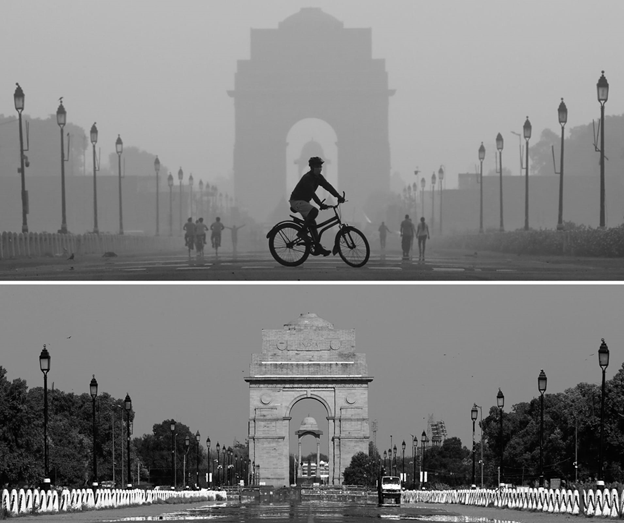
\includegraphics[width=0.6\linewidth]{images/air_pollution_greyscale} 

}

\caption{The India Gate in New Delhi, India}\label{fig:unnamed-chunk-1}
\end{figure}

Have high population-density U.S. cities seen the same improved air quality conditions? To study this question, data was gathered from the U.S. Environmental Protection Agency (EPA) AirData website which records the ozone (O3) and fine particulate matter (PM2.5) values for cities across the U.S. These measures are used to calculate an air quality index (AQI) score for each city each day of the year. Thirty-three of the most densely populated U.S. cities were selected and the AQI score recorded for April 20, 2020 as well as the five-year median AQI score for April 20th (2015 - 2019). Note that higher AQI scores indicate worse air quality.

\begin{center}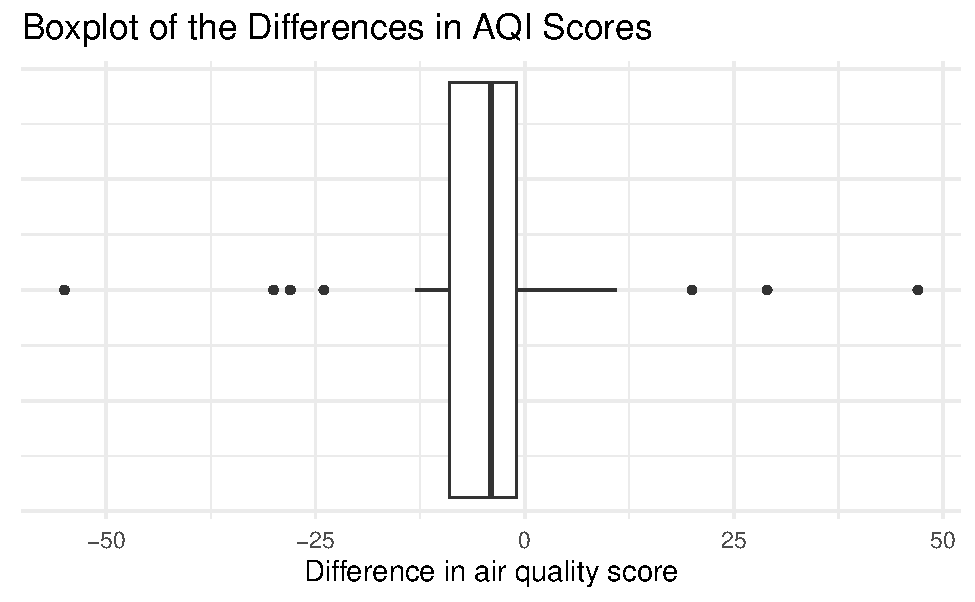
\includegraphics[width=0.6\linewidth]{08-paired_files/figure-latex/unnamed-chunk-3-1} \end{center}

\begin{longtable}[]{@{}ccll@{}}
\toprule
& Mean & Standard deviation & Sample size\tabularnewline
\midrule
\endhead
Current & \(\bar{x}_1\) = 47.394 & \(s_1\) = 14.107 & \(n_1\) = 33\tabularnewline
5 Year Median & \(\bar{x}_2\) = 51.545 & \(s_2\) = 17.447 & \(n_2\) = 33\tabularnewline
Differences & \(\bar{x}_d\) = -4.152 & \(s_d\) = 17.096 & \(n_d\) = 33\tabularnewline
\bottomrule
\end{longtable}

\newpage

\hypertarget{vocabulary-review}{%
\subsection{Vocabulary review}\label{vocabulary-review}}

\begin{enumerate}
\def\labelenumi{\arabic{enumi}.}
\tightlist
\item
  What is the sample size?
\end{enumerate}

\vspace{0.5in}

\begin{enumerate}
\def\labelenumi{\arabic{enumi}.}
\setcounter{enumi}{1}
\tightlist
\item
  Identify the variables in this study. What role do each have?
\end{enumerate}

\vspace{.8in}

\begin{enumerate}
\def\labelenumi{\arabic{enumi}.}
\setcounter{enumi}{2}
\tightlist
\item
  Why is this treated as a paired study design and not two independent samples?
\end{enumerate}

\vspace{1in}

\begin{enumerate}
\def\labelenumi{\arabic{enumi}.}
\setcounter{enumi}{3}
\tightlist
\item
  Is this an experiment or observational study? Justify your answer.
\end{enumerate}

\vspace{0.3in}

\hypertarget{ask-a-research-question}{%
\subsection{Ask a research question}\label{ask-a-research-question}}

\begin{enumerate}
\def\labelenumi{\arabic{enumi}.}
\setcounter{enumi}{4}
\tightlist
\item
  What are the two competing possibilities to run a hypothesis test for this study?
\end{enumerate}

\vspace{1in}

\begin{enumerate}
\def\labelenumi{\arabic{enumi}.}
\setcounter{enumi}{5}
\tightlist
\item
  Write the null hypothesis in words.
\end{enumerate}

\vspace{1in}

\begin{enumerate}
\def\labelenumi{\arabic{enumi}.}
\setcounter{enumi}{6}
\tightlist
\item
  What is the research question?
\end{enumerate}

\vspace{1in}

\begin{enumerate}
\def\labelenumi{\arabic{enumi}.}
\setcounter{enumi}{7}
\tightlist
\item
  Write the alternative hypothesis in notation.
\end{enumerate}

\vspace{1in}

\newpage

\hypertarget{summarize-and-visualize-the-data}{%
\subsection{Summarize and visualize the data}\label{summarize-and-visualize-the-data}}

\begin{enumerate}
\def\labelenumi{\arabic{enumi}.}
\setcounter{enumi}{8}
\tightlist
\item
  Report the summary statistic for the data.
\end{enumerate}

\vspace{0.3in}

\begin{enumerate}
\def\labelenumi{\arabic{enumi}.}
\setcounter{enumi}{9}
\tightlist
\item
  What notation is used for the value in question 9?
\end{enumerate}

\vspace{0.3in}

\hypertarget{use-statistical-inferential-methods-to-draw-inferences-from-the-data}{%
\subsection{Use statistical inferential methods to draw inferences from the data}\label{use-statistical-inferential-methods-to-draw-inferences-from-the-data}}

To simulate the null distribution we will use a bootstrapping method. Recall that the null distribution must be created under the assumption that the null hypothesis is true. Therefore, before bootstrapping we will need to shift each data point by the difference \(\mu_0 - \bar{x}\). This will ensure that the mean of the shifted data is \(\mu_0\) and that the simulated null distribution will be centered at the null value.

\begin{enumerate}
\def\labelenumi{\arabic{enumi}.}
\setcounter{enumi}{10}
\tightlist
\item
  Calculate the difference \(\mu_0 - \bar{x}\). Will we need to shift the data up or down?
\end{enumerate}

\vspace{.7in}

\begin{enumerate}
\def\labelenumi{\arabic{enumi}.}
\setcounter{enumi}{11}
\tightlist
\item
  Use the provided \texttt{R} markdown file and enter the calculated value from question 11 for xx to simulate the null distribution and enter the summary statistic from question 9 for yy to find the p-value.
\end{enumerate}

\begin{Shaded}
\begin{Highlighting}[]
    \KeywordTok{paired\_test}\NormalTok{(}\DataTypeTok{data =}\NormalTok{ Air}\OperatorTok{$}\NormalTok{Difference,   }\CommentTok{\#Vector of differences or data set with column for each group}
            \DataTypeTok{shift =}\NormalTok{ xx,   }\CommentTok{\#Shift needed for bootstrap hypothesis test}
            \DataTypeTok{as\_extreme\_as =}\NormalTok{ yy,  }\CommentTok{\#Observed statistic}
            \DataTypeTok{direction =} \StringTok{"less"}\NormalTok{,  }\CommentTok{\#Direction of alternative}
            \DataTypeTok{number\_repetitions =} \DecValTok{1000}\NormalTok{,  }\CommentTok{\#Number of simulated samples for null distribution}
            \DataTypeTok{which\_first =} \DecValTok{1}\NormalTok{)  }\CommentTok{\#Not needed when using calculated differences}
\end{Highlighting}
\end{Shaded}

\begin{enumerate}
\def\labelenumi{\arabic{enumi}.}
\setcounter{enumi}{12}
\tightlist
\item
  Sketch the null distribution created in Question 12 here.
\end{enumerate}

\vspace{2in}

\begin{enumerate}
\def\labelenumi{\arabic{enumi}.}
\setcounter{enumi}{13}
\tightlist
\item
  Explain why the null distribution is centered at zero.
\end{enumerate}

\vspace{.5in}

\begin{enumerate}
\def\labelenumi{\arabic{enumi}.}
\setcounter{enumi}{14}
\tightlist
\item
  What proportion of samples are at or less than the sample mean difference in AQI Scores for current scores minus 5 year median scores?
\end{enumerate}

\newpage

\begin{enumerate}
\def\labelenumi{\arabic{enumi}.}
\setcounter{enumi}{15}
\tightlist
\item
  Interpret the p-value in the context of the problem.
\end{enumerate}

\vspace{1in}

\begin{enumerate}
\def\labelenumi{\arabic{enumi}.}
\setcounter{enumi}{16}
\tightlist
\item
  How much evidence does this provide for improved air quality in US cities?
\end{enumerate}

\vspace{.5in}

\begin{enumerate}
\def\labelenumi{\arabic{enumi}.}
\setcounter{enumi}{17}
\tightlist
\item
  Write out the parameter of interest in context of the study.
\end{enumerate}

\vspace{1in}

The following \texttt{R} code creates a bootstrap distribution showing 1000 simulations of the mean difference.

\begin{Shaded}
\begin{Highlighting}[]
\KeywordTok{paired\_bootstrap\_CI}\NormalTok{(}\DataTypeTok{data =}\NormalTok{ Air}\OperatorTok{$}\NormalTok{Difference, }\CommentTok{\#Enter vector of differences}
                    \DataTypeTok{number\_repetitions =} \DecValTok{1000}\NormalTok{, }\CommentTok{\#Number of bootstrap samples for CI}
                    \DataTypeTok{confidence\_level =} \FloatTok{0.99}\NormalTok{,  }\CommentTok{\#Confidence level in decimal form}
                    \DataTypeTok{which\_first =} \DecValTok{1}\NormalTok{)  }\CommentTok{\#Not needed when entering vector of differences}
\end{Highlighting}
\end{Shaded}

\begin{center}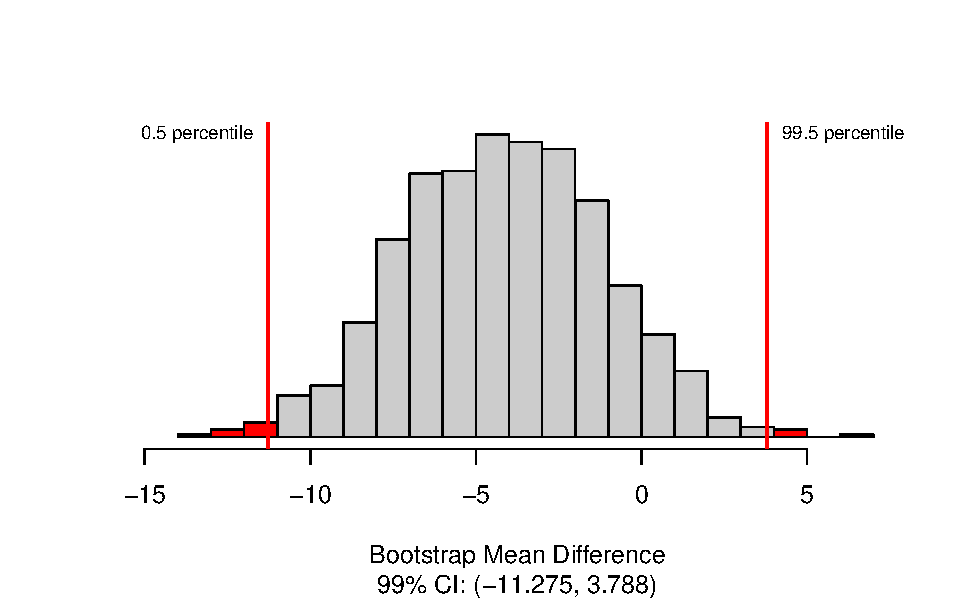
\includegraphics[width=0.7\linewidth]{08-paired_files/figure-latex/unnamed-chunk-6-1} \end{center}

\begin{enumerate}
\def\labelenumi{\arabic{enumi}.}
\setcounter{enumi}{18}
\tightlist
\item
  Use the bootstrapped distribution above to find a 99\% confidence interval for the parameter of interest. Report the confidence interval in interval notation.
\end{enumerate}

\vspace{.3in}

\hypertarget{communicate-the-results-and-answer-the-research-question.}{%
\subsection{Communicate the results and answer the research question.}\label{communicate-the-results-and-answer-the-research-question.}}

\begin{enumerate}
\def\labelenumi{\arabic{enumi}.}
\setcounter{enumi}{19}
\tightlist
\item
  Interpret the 99\% confidence interval in the context of the problem.
\end{enumerate}

\newpage

\begin{enumerate}
\def\labelenumi{\arabic{enumi}.}
\setcounter{enumi}{20}
\tightlist
\item
  Write a paragraph summarizes the results of this study. Be sure to include:
\end{enumerate}

\begin{itemize}
\item
  Summary statistic
\item
  P-value and interpretation
\item
  Conclusion (written to answer the research question)
\item
  Confidence interval and interpretation
\item
  Scope of inference
\end{itemize}

\vspace{3in}

\hypertarget{revisit-and-look-forward}{%
\subsection{Revisit and look forward}\label{revisit-and-look-forward}}

\begin{enumerate}
\def\labelenumi{\arabic{enumi}.}
\setcounter{enumi}{21}
\tightlist
\item
  Would it be possible to design an experiment to determine if the changed human behavior due to the COVID-19 pandemic causes a decrease in air pollution? Explain.
  \vspace{1in}
\end{enumerate}

\hypertarget{additional-notes}{%
\section{Additional notes}\label{additional-notes}}

Use this space to summarize your thoughts and take additional notes on today's activity.

\hypertarget{weather-patterns-and-record-snowfall}{%
\chapter{Weather Patterns and Record Snowfall}\label{weather-patterns-and-record-snowfall}}

\newcommand\latexcode[1]{#1}

\hypertarget{learning-objectives}{%
\section{Learning objectives}\label{learning-objectives}}

\begin{itemize}
\item
  Write out the null and alternative hypothesis for one categorical and one quantitative variable
\item
  Calculate and carry-out simulation based hypothesis test for a difference in means
\item
  Interpret and evaluate a p-value
\item
  Find a bootstap confidence interval for a difference in means
\item
  Use a confidence interval to determine the conclusion of a hypothesis test
\end{itemize}

\hypertarget{terminology-review}{%
\section{Terminology review}\label{terminology-review}}

In today's activity, we will use simulation-based methods to analyze two independent quantitative variables. Some terms covered in this activity are:

\begin{itemize}
\item
  Independent groups
\item
  Difference in means
\end{itemize}

To review these concepts, see Section 6.3 in the textbook.

\hypertarget{weather-patterns-and-record-snowfall-1}{%
\section{Weather Patterns and Record snowfall}\label{weather-patterns-and-record-snowfall-1}}

In the winter of 2018-2019, Bozeman had a record snowfall which resulted in the collapse of two flat-roofed buildings on the MSU campus. A writer for the Washington Post predicted the heavy snowfall for 2018-2019 due to the El Ni\~{n}o weather pattern that occurred in that season. A meteorologist in Montana wanted to see if the weather pattern really was associated with total snowfall. She obtained historical data from 44 years on the weather pattern (El Ni\~{n}o or La Ni\~{n}a) and snowfall (in inches) at the Billings Weather Station.

\begin{Shaded}
\begin{Highlighting}[]
\KeywordTok{ggplot}\NormalTok{(}\DataTypeTok{data =}\NormalTok{ Snow,}
       \KeywordTok{aes}\NormalTok{(}\DataTypeTok{x =}\NormalTok{ WeatherPattern, }\DataTypeTok{y =}\NormalTok{ Snowfall)) }\OperatorTok{+}
\StringTok{    }\KeywordTok{geom\_boxplot}\NormalTok{() }\OperatorTok{+}\StringTok{ }
\StringTok{    }\KeywordTok{labs}\NormalTok{(}\DataTypeTok{title =} \StringTok{"Snowfall by weather pattern"}\NormalTok{,}
         \DataTypeTok{x =} \StringTok{"Weather pattern"}\NormalTok{) }\OperatorTok{+}
\StringTok{    }\KeywordTok{coord\_flip}\NormalTok{()}
\end{Highlighting}
\end{Shaded}

\begin{center}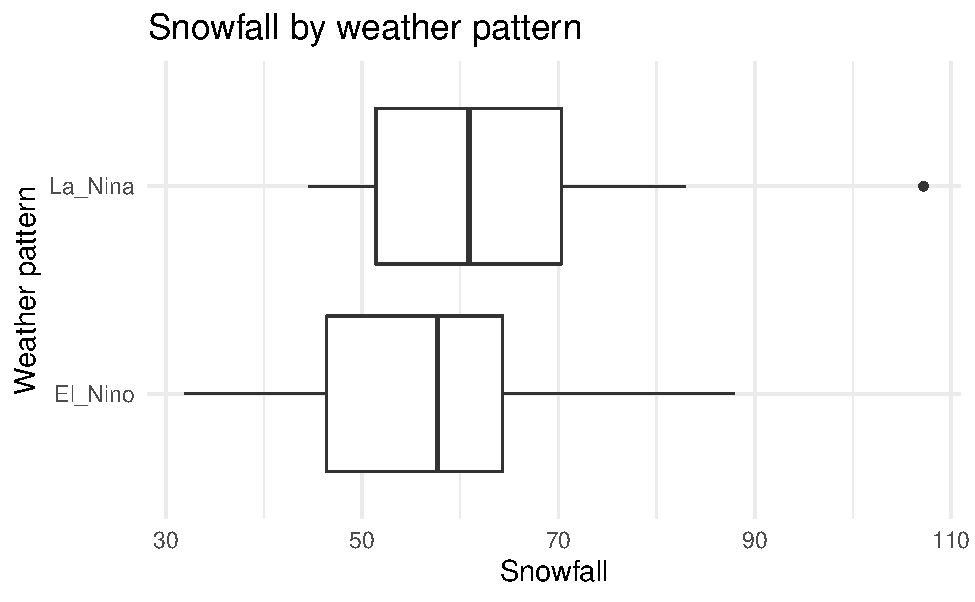
\includegraphics[width=0.6\linewidth]{09-inference-2quant_files/figure-latex/unnamed-chunk-2-1} \end{center}

\begin{Shaded}
\begin{Highlighting}[]
\KeywordTok{favstats}\NormalTok{(Snowfall}\OperatorTok{\textasciitilde{}}\NormalTok{WeatherPattern, }\DataTypeTok{data=}\NormalTok{Snow)}
\end{Highlighting}
\end{Shaded}

\begin{verbatim}
#>   WeatherPattern  min   Q1 median   Q3   max     mean       sd  n missing
#> 1        El_Nino 31.9 46.4   57.7 64.3  87.9 56.23043 13.00823 23       0
#> 2        La_Nina 44.5 51.4   60.9 70.3 107.2 63.13333 15.48626 21       0
\end{verbatim}

\hypertarget{quantitative-variables-review}{%
\subsection{Quantitative variables review}\label{quantitative-variables-review}}

\begin{enumerate}
\def\labelenumi{\arabic{enumi}.}
\tightlist
\item
  The two variables assessed in this study are the type of weather pattern and snowfall. Identify the role for each variable (explanatory, response).
\end{enumerate}

\vspace{1in}

\begin{enumerate}
\def\labelenumi{\arabic{enumi}.}
\setcounter{enumi}{1}
\tightlist
\item
  Which group (El Ni\~{n}o or La Ni\~{n}a) has the highest center? Explain which measure you are using.
\end{enumerate}

\vspace{1in}

\begin{enumerate}
\def\labelenumi{\arabic{enumi}.}
\setcounter{enumi}{2}
\tightlist
\item
  Using the side-by-side boxplots, which group has the largest spread? How did you make that choice?
\end{enumerate}

\vspace{1in}

\begin{enumerate}
\def\labelenumi{\arabic{enumi}.}
\setcounter{enumi}{3}
\tightlist
\item
  Is this an experiment or an observational study? Explain your reasoning.
\end{enumerate}

\vspace{1in}

\begin{enumerate}
\def\labelenumi{\arabic{enumi}.}
\setcounter{enumi}{4}
\tightlist
\item
  Is this a paired data set or two independent groups? Explain your answer.
\end{enumerate}

\vspace{1in}

\hypertarget{ask-a-research-question.}{%
\subsection{Ask a research question.}\label{ask-a-research-question.}}

\begin{enumerate}
\def\labelenumi{\arabic{enumi}.}
\setcounter{enumi}{5}
\tightlist
\item
  Write out the parameter of interest in context of the study. Use proper notation and be sure to define your subscripts. Use El Ni\~{n}o minus La Ni\~{n}a as the order of subtraction.
\end{enumerate}

\vspace{1in}

\begin{enumerate}
\def\labelenumi{\arabic{enumi}.}
\setcounter{enumi}{6}
\tightlist
\item
  What are the two competing possibilities we will evaluate in this study?
\end{enumerate}

\vspace{1in}

\begin{enumerate}
\def\labelenumi{\arabic{enumi}.}
\setcounter{enumi}{7}
\tightlist
\item
  Identify which of your answers in question 7 is the null hypothesis and which is the alternative hypothesis.
\end{enumerate}

\vspace{1in}

\hypertarget{summarize-and-visualize-the-data}{%
\subsection{Summarize and visualize the data}\label{summarize-and-visualize-the-data}}

\begin{enumerate}
\def\labelenumi{\arabic{enumi}.}
\setcounter{enumi}{8}
\tightlist
\item
  Calculate the summary statistic. Use El Ni\~{n}o minus La Ni\~{n}a as the order of subtraction. What is the appropriate notation for the statistic?
\end{enumerate}

\vspace{0.5in}

\hypertarget{use-statistical-inferential-methods-to-draw-inferences-from-the-data}{%
\subsection{Use statistical inferential methods to draw inferences from the data}\label{use-statistical-inferential-methods-to-draw-inferences-from-the-data}}

Remember that the null distribution is created based on the assumption the null hypothesis is true. In this study, we asssume there is no association between variables. This means that a snowfall value could be in either an El Ni\~{n}o year or a La Ni\~{n}a year.

To demonstrate this your instructor will use cards to represent the sample.

\begin{enumerate}
\def\labelenumi{\arabic{enumi}.}
\setcounter{enumi}{9}
\tightlist
\item
  How many cards will we start with?
\end{enumerate}

\vspace{0.5in}

\begin{enumerate}
\def\labelenumi{\arabic{enumi}.}
\setcounter{enumi}{10}
\tightlist
\item
  What will we write on each card?
\end{enumerate}

\vspace{0.5in}

\begin{enumerate}
\def\labelenumi{\arabic{enumi}.}
\setcounter{enumi}{11}
\tightlist
\item
  Next we will mix the cards together and shuffle into two piles. How many cards will go into each pile? What should we label the piles?
\end{enumerate}

\vspace{1in}

\begin{enumerate}
\def\labelenumi{\arabic{enumi}.}
\setcounter{enumi}{12}
\tightlist
\item
  What value is calculated from the cards and plotted on the null distribution?
\end{enumerate}

\vspace{1in}

\begin{enumerate}
\def\labelenumi{\arabic{enumi}.}
\setcounter{enumi}{13}
\tightlist
\item
  Once we create a null distribution of 1000 simulations, at what value do you expect the distribution to be centered? Explain your answer.
\end{enumerate}

\vspace{1in}

\textbf{Simulation method}

\begin{enumerate}
\def\labelenumi{\arabic{enumi}.}
\setcounter{enumi}{14}
\tightlist
\item
  Using the provided \texttt{R} markdown file, enter the values for the variables, dataset, first in subtraction, number of simulations, observed statistic, and direction of the alternative hypothesis.
\end{enumerate}

\begin{Shaded}
\begin{Highlighting}[]
\KeywordTok{two\_mean\_test}\NormalTok{(RESPONSE}\OperatorTok{\textasciitilde{}}\NormalTok{PREDICTOR, }\DataTypeTok{data =}\NormalTok{ DATASET,  }\CommentTok{\#Variables and data}
                    \DataTypeTok{first\_in\_subtraction =} \StringTok{"VALUE"}\NormalTok{, }\CommentTok{\#First value in order of subtraction}
                    \DataTypeTok{number\_repetitions =} \CommentTok{\#\#\#,  \#Number of simulations}
                    \DataTypeTok{as\_extreme\_as =} \CommentTok{\#\#\#,  \#Observed statistic}
                    \DataTypeTok{direction =} \StringTok{"??"}\NormalTok{)  }\CommentTok{\#Direction of alternative: "greater", "less", or "two{-}sided"}
\end{Highlighting}
\end{Shaded}

\vspace{1in}

\begin{enumerate}
\def\labelenumi{\arabic{enumi}.}
\setcounter{enumi}{15}
\tightlist
\item
  Report the p-value. How much evidence does the p-value provide against the null hypothesis?
\end{enumerate}

\vspace{1in}

\begin{enumerate}
\def\labelenumi{\arabic{enumi}.}
\setcounter{enumi}{16}
\tightlist
\item
  Using bootstrapping find a 90\% confidence interval. Use the provided \texttt{R} markdown file. Enter the variables, first in subtraction, number of repetitions, and the confidence level.
\end{enumerate}

\begin{Shaded}
\begin{Highlighting}[]
\KeywordTok{two\_mean\_bootstrap\_CI}\NormalTok{(RESPONSE}\OperatorTok{\textasciitilde{}}\NormalTok{EXPLANATORY, }\DataTypeTok{data =}\NormalTok{ DATASET,  }\CommentTok{\#Variables and data}
                      \DataTypeTok{first\_in\_subtraction =} \StringTok{"VALUE"}\NormalTok{, }\CommentTok{\#First value in order of subtraction}
                      \DataTypeTok{number\_repetitions =} \CommentTok{\#\#\#,  \#Number of simulations}
                      \DataTypeTok{confidence\_level =} \CommentTok{\#\#)}
\end{Highlighting}
\end{Shaded}

\begin{enumerate}
\def\labelenumi{\arabic{enumi}.}
\setcounter{enumi}{17}
\tightlist
\item
  Interpret the interval you calculated in Question 17.
\end{enumerate}

\vspace{1in}

\hypertarget{communicate-the-results-and-answer-the-research-question}{%
\subsection{Communicate the results and answer the research question}\label{communicate-the-results-and-answer-the-research-question}}

\begin{enumerate}
\def\labelenumi{\arabic{enumi}.}
\setcounter{enumi}{18}
\tightlist
\item
  Write a paragraph summarizing the results of the study. Be sure to include:
\end{enumerate}

\begin{itemize}
\item
  Summary statistic
\item
  P-value and interpretation
\item
  Conclusion (written to answer the research question)
\item
  Confidence interval and interpretation
\item
  Scope of inference
\end{itemize}

\vspace{3in}

\hypertarget{revisit-and-look-rorward}{%
\subsection{Revisit and look rorward}\label{revisit-and-look-rorward}}

\begin{enumerate}
\def\labelenumi{\arabic{enumi}.}
\setcounter{enumi}{19}
\tightlist
\item
  Would the results from the theory-based test match the results we saw with the simulation? Explain why or why not.
\end{enumerate}

\vspace{1in}

\begin{enumerate}
\def\labelenumi{\arabic{enumi}.}
\setcounter{enumi}{20}
\tightlist
\item
  If we had data on 45 La Ni\~{n}a years and 47 El Ni\~{n}o years and found a similar summary statistic, what would happen to the p-value? The width of the confidence interval? The power of the test?
\end{enumerate}

\vspace{1in}

\hypertarget{additional-notes}{%
\section{Additional notes}\label{additional-notes}}

Use this space to summarize your thoughts and take additional notes on today's activity.

\hypertarget{hand-dexterity}{%
\chapter{Hand Dexterity}\label{hand-dexterity}}

\hypertarget{learning-outcomes}{%
\section{Learning outcomes}\label{learning-outcomes}}

\begin{itemize}
\item
  Given a research question, construct the null and alternative hypotheses
  in words and using appropriate statistical symbols
\item
  Describe and perform theory-based hypothesis tests for the slope
\item
  Interpret and evaluate a p-value
\item
  Construct and interpret a theory-based confidence interval for slope
\item
  Use a confidence interval to determine the conclusion of a hypothesis test
\end{itemize}

\hypertarget{terminology-review}{%
\section{Terminology review}\label{terminology-review}}

In today's activity, we will use theory-based hypothesis tests and confidence intervals for a linear regression slope. Some terms covered in this activity are:

\begin{itemize}
\item
  Correlation
\item
  Slope
\item
  Regression line
\end{itemize}

To review these concepts, see Chapters 3 and 7 in the textbook.

\hypertarget{hand-dexterity-1}{%
\section{Hand dexterity}\label{hand-dexterity-1}}

Physical therapists often evaluate manual (hand) dexterity by having patients complete simple tasks, such as moving pegs on a board or threading objects through holes. Researchers want to examine the manual dexterity of children as part of a follow-up study of a test originally designed for adults to see how manual dexterity changes with age. In this test, 174 participants were given a board with 16 pegs, each in their own hole, arranged in a 4x4 grid. Participants were instructed to pick up the peg with one hand, flip it over by rotating their wrist, then reinsert it in the same hole. Using this test, researchers want to know if as people age the speed at which they can flip all 16 pegs increases.

The variables in this dataset consist of the following:

\begin{itemize}
\item
  \textbf{time:} Recorded time to flip all 16 pegs, measured in seconds.
\item
  \textbf{speed:} The average speed to flip a peg for each participant (seconds per peg).
\item
  \textbf{age:} Age of the participants, measured in years.
\item
  \textbf{dominant:} Whether the participant's dominant hand was used, coded as 0 for no, 1 for yes.
\item
  \textbf{gender:} The participant's gender, recorded as a binary variable, 0 for male, 1 for female.
\item
  \textbf{HD:} The dominant hand of the participant, recorded as ``R'' for right hand, ``L'' for left hand.
\item
  \textbf{handUsed:} Which hand the participant used to complete the test, recorded as ``R'' for right hand, ``L'' for left hand.
\end{itemize}

\emph{Data source: Hand Dexterity in Children: Administration and Normative Values of the Functional Dexterity Test (FDT), Gogola, G., et al., 2013}

\hypertarget{vocabulary-review}{%
\subsection{Vocabulary review}\label{vocabulary-review}}

\begin{enumerate}
\def\labelenumi{\arabic{enumi}.}
\tightlist
\item
  Explain why regression methods are appropriate to use to address the researchers' question. Make sure you clearly define the variables of interest in your explanation and their roles.
\end{enumerate}

\vspace{1in}

\begin{enumerate}
\def\labelenumi{\arabic{enumi}.}
\setcounter{enumi}{1}
\tightlist
\item
  What is the scope of inference for this study? Explain your answer.
\end{enumerate}

\vspace{1in}

\begin{enumerate}
\def\labelenumi{\arabic{enumi}.}
\setcounter{enumi}{2}
\tightlist
\item
  Use the provided \texttt{R} markdown file to create a scatterplot to examine the relationship between the speed at which a participant can flip a peg and the age of the participant by filling in the variable names (`speed' and `age') for xxx and xxxx. Provide this plot. Based on your plot, does it appear that there is a relationship between \texttt{age} and \texttt{speed}? Note: \texttt{age} should be on the x-axis.
\end{enumerate}

\begin{Shaded}
\begin{Highlighting}[]
    \KeywordTok{ggplot}\NormalTok{(}\DataTypeTok{data =}\NormalTok{ hands,   }\CommentTok{\#This is the data set}
       \KeywordTok{aes}\NormalTok{(}\DataTypeTok{x =}\NormalTok{ xxx, }\DataTypeTok{y =}\NormalTok{ xxxx))}\OperatorTok{+}\StringTok{  }\CommentTok{\#Specify variables}
\StringTok{    }\KeywordTok{geom\_point}\NormalTok{() }\OperatorTok{+}\StringTok{  }\CommentTok{\#Add scatterplot of points}
\StringTok{    }\KeywordTok{labs}\NormalTok{(}\DataTypeTok{x =} \StringTok{"Age (yrs)"}\NormalTok{,  }\CommentTok{\#Label x{-}axis}
       \DataTypeTok{y =} \StringTok{"Speed (sec/peg)"}\NormalTok{,  }\CommentTok{\#Label y{-}axis}
       \DataTypeTok{title =} \StringTok{"Scatterplot of Age vs. Speed"}\NormalTok{) }\OperatorTok{+}\StringTok{ }\CommentTok{\#Be sure to tile your plots}
\StringTok{    }\KeywordTok{geom\_smooth}\NormalTok{(}\DataTypeTok{method =} \StringTok{"lm"}\NormalTok{, }\DataTypeTok{se =} \OtherTok{FALSE}\NormalTok{)  }\CommentTok{\#Add regression line}
\end{Highlighting}
\end{Shaded}

\vspace{2in}

\begin{enumerate}
\def\labelenumi{\arabic{enumi}.}
\setcounter{enumi}{3}
\tightlist
\item
  Describe the features of the plot you created in Question 3.
\end{enumerate}

\vspace{1in}

If you indicated there are potential outliers, which points are they?

\vspace{0.5in}

\hypertarget{conditions-for-the-least-squares-line}{%
\subsection{Conditions for the least squares line}\label{conditions-for-the-least-squares-line}}

When performing inference on a least squares line, the follow conditions are generally required

\begin{itemize}
\tightlist
\item
  Linearity: the data should follow a linear trend
\item
  Nearly normal residuals: residuals must be nearly normal
\item
  Constant variability: the variability of points around the least squares line remains roughly constant
\item
  Independent observations: individual data points must be independent
\end{itemize}

The scatterplot and the residual plots will be used to assess the conditions for approximating the data with the \(t\)-distribution.

\begin{center}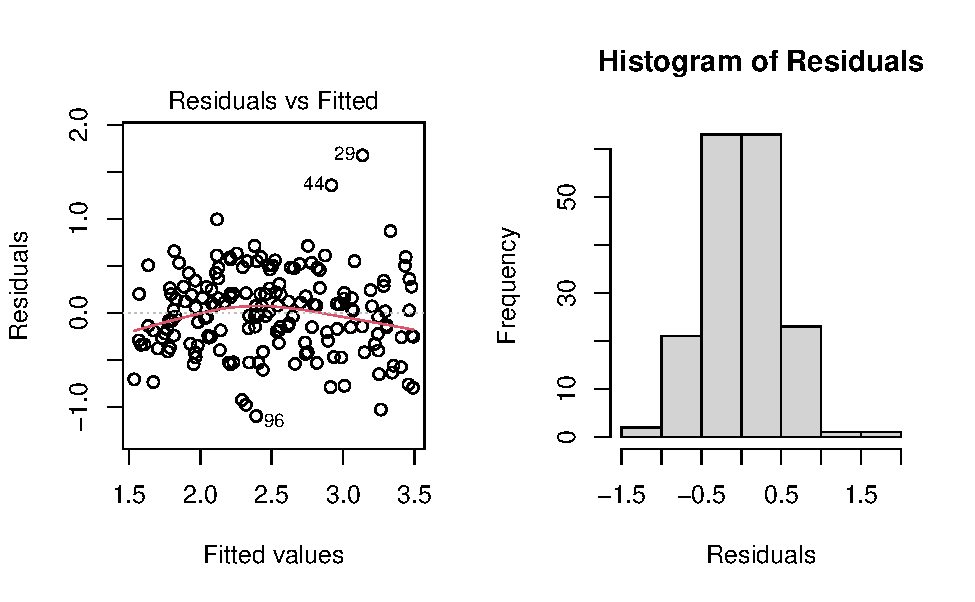
\includegraphics[width=0.7\linewidth]{10-regression_files/figure-latex/unnamed-chunk-3-1} \end{center}

\begin{enumerate}
\def\labelenumi{\arabic{enumi}.}
\setcounter{enumi}{4}
\tightlist
\item
  Are the conditions met to approximate the \(t\)-distribution?
\end{enumerate}

\vspace{1in}

\hypertarget{ask-a-research-question}{%
\subsection{Ask a research question}\label{ask-a-research-question}}

\begin{enumerate}
\def\labelenumi{\arabic{enumi}.}
\setcounter{enumi}{5}
\tightlist
\item
  Write out the null hypothesis in words.
\end{enumerate}

\vspace{1in}

\begin{enumerate}
\def\labelenumi{\arabic{enumi}.}
\setcounter{enumi}{6}
\tightlist
\item
  Using the research question, write the alternative hypothesis in notation.
\end{enumerate}

\vspace{0.5in}

\hypertarget{summarize-and-visualize-the-data}{%
\subsection{Summarize and visualize the data}\label{summarize-and-visualize-the-data}}

Using the provided \texttt{R} markdown file, enter the response variable into the linear model function for xxx and the explanatory variable for xxxx to get the linear model output.

\begin{Shaded}
\begin{Highlighting}[]
\NormalTok{    lm.hand \textless{}{-}}\StringTok{ }\KeywordTok{lm}\NormalTok{(xxx}\OperatorTok{\textasciitilde{}}\NormalTok{xxxx, }\DataTypeTok{data=}\NormalTok{hands) }\CommentTok{\#lm(response\textasciitilde{}explanatory)}
    \KeywordTok{summary}\NormalTok{(lm.hand)}\OperatorTok{$}\NormalTok{coefficients}
\end{Highlighting}
\end{Shaded}

\begin{enumerate}
\def\labelenumi{\arabic{enumi}.}
\setcounter{enumi}{7}
\tightlist
\item
  Using the output from the evaluated \texttt{R} code above, write the equation of the regression line.
\end{enumerate}

\vspace{1in}

\begin{enumerate}
\def\labelenumi{\arabic{enumi}.}
\setcounter{enumi}{8}
\tightlist
\item
  Interpret the slope in context of the problem.
\end{enumerate}

\vspace{1in}

\begin{enumerate}
\def\labelenumi{\arabic{enumi}.}
\setcounter{enumi}{9}
\tightlist
\item
  Using your estimated line of best fit, predict the per peg speed for a participant who was 9.18 years old. Show all work.
\end{enumerate}

\vspace{1in}

\begin{enumerate}
\def\labelenumi{\arabic{enumi}.}
\setcounter{enumi}{10}
\tightlist
\item
  Calculate the residual associated with the observation (9.18, 2.95), using your estimated regression line from question 8.
\end{enumerate}

\vspace{1in}

\hypertarget{use-statistical-inferential-methods-to-draw-inferences-from-the-data}{%
\subsection{Use statistical inferential methods to draw inferences from the data}\label{use-statistical-inferential-methods-to-draw-inferences-from-the-data}}

To find the value of the test statistic to test the slope we will use,

\[
T = \frac{\mbox{slope estimate}}{SE} = \frac{b_1}{SE(b_1)}
\]

We will use the linear model output above to get the estimate for slope and standard error.

\begin{enumerate}
\def\labelenumi{\arabic{enumi}.}
\setcounter{enumi}{11}
\tightlist
\item
  Calculate the test statistic for slope. Identify where this calculated value is in the linear model output.
\end{enumerate}

\vspace{1in}

\begin{enumerate}
\def\labelenumi{\arabic{enumi}.}
\setcounter{enumi}{12}
\tightlist
\item
  Interpret the test statistic in context of the problem.
\end{enumerate}

\vspace{1in}

\begin{enumerate}
\def\labelenumi{\arabic{enumi}.}
\setcounter{enumi}{13}
\tightlist
\item
  Using the linear model output, report the p-value for the test of significance.
\end{enumerate}

\vspace{0.5in}

\begin{enumerate}
\def\labelenumi{\arabic{enumi}.}
\setcounter{enumi}{14}
\tightlist
\item
  Based on the p-value, how much evidence is there against the null hypothesis?
\end{enumerate}

\vspace{0.5in}

Recall that a confidence interval is calculated by adding and subtracting the margin of error to the point estimate.\\
\[\mbox{point estimate}\pm t^*SE(estimate)\]
\[b_1 \pm t^* SE(b_1)\]

The \(t^*\) multiplier comes from the \(t\)-distribution with \(n-2\) df.

\begin{Shaded}
\begin{Highlighting}[]
\KeywordTok{qt}\NormalTok{(}\FloatTok{0.95+0.025}\NormalTok{, }\DecValTok{172}\NormalTok{) }\CommentTok{\#95\% t* multiplier }
\CommentTok{\#\textgreater{} [1] 1.973852}
\end{Highlighting}
\end{Shaded}

\begin{enumerate}
\def\labelenumi{\arabic{enumi}.}
\setcounter{enumi}{15}
\tightlist
\item
  Calculate the 95\% confidence interval for the true slope.
  \vspace{1in}
\end{enumerate}

\hypertarget{communicate-the-results-and-answer-the-research-question}{%
\subsection{Communicate the results and answer the research question}\label{communicate-the-results-and-answer-the-research-question}}

\begin{enumerate}
\def\labelenumi{\arabic{enumi}.}
\setcounter{enumi}{16}
\tightlist
\item
  Based on the p-value, write a conclusion in context of the problem.
\end{enumerate}

\vspace{1in}

\begin{enumerate}
\def\labelenumi{\arabic{enumi}.}
\setcounter{enumi}{17}
\tightlist
\item
  Interpret the 95\% confidence interval in context of the problem.
\end{enumerate}

\vspace{1in}

\begin{enumerate}
\def\labelenumi{\arabic{enumi}.}
\setcounter{enumi}{18}
\tightlist
\item
  Summarize the results of the study in a written paragraph. Be sure to include.
\end{enumerate}

\begin{itemize}
\item
  Summary statistic
\item
  Test statistic and interpretation
\item
  P-value and interpretation
\item
  Confidence interval and interpretation
\item
  Conclusion (written to answer the research question)
\item
  Scope of inference
\end{itemize}

\vspace{2in}

\hypertarget{revisit-and-look-forward}{%
\subsection{Revisit and look forward}\label{revisit-and-look-forward}}

\begin{enumerate}
\def\labelenumi{\arabic{enumi}.}
\setcounter{enumi}{19}
\tightlist
\item
  Is there an effect due to gender on the linear relationship between age and speed? Explain your answer using the scatterplot below.
\end{enumerate}

\begin{Shaded}
\begin{Highlighting}[]
\KeywordTok{ggplot}\NormalTok{(}\DataTypeTok{data =}\NormalTok{ hands,   }\CommentTok{\#This is the data set}
       \KeywordTok{aes}\NormalTok{(}\DataTypeTok{x =}\NormalTok{ age, }\DataTypeTok{y =}\NormalTok{ speed, }\DataTypeTok{color =}\NormalTok{ dominant))}\OperatorTok{+}\StringTok{  }\CommentTok{\#Specify variables}
\StringTok{  }\KeywordTok{geom\_point}\NormalTok{(}\KeywordTok{aes}\NormalTok{(}\DataTypeTok{pch =}\NormalTok{ dominant)) }\OperatorTok{+}\StringTok{  }\CommentTok{\#Add scatterplot of points}
\StringTok{  }\KeywordTok{labs}\NormalTok{(}\DataTypeTok{x =} \StringTok{"Age (yrs)"}\NormalTok{,  }\CommentTok{\#Label x{-}axis}
       \DataTypeTok{y =} \StringTok{"Speed (sec/peg)"}\NormalTok{,  }\CommentTok{\#Label y{-}axis}
       \DataTypeTok{legend =} \StringTok{"Dominant hand"}\NormalTok{,  }\CommentTok{\#Label your legend}
       \DataTypeTok{title =} \StringTok{"Scatterplot of Age vs. Speed"}\NormalTok{) }\OperatorTok{+}\StringTok{ }\CommentTok{\#Be sure to tile your plots}
\StringTok{  }\KeywordTok{geom\_smooth}\NormalTok{(}\DataTypeTok{method =} \StringTok{"lm"}\NormalTok{, }\DataTypeTok{se =} \OtherTok{FALSE}\NormalTok{) }\OperatorTok{+}\StringTok{  }\CommentTok{\#Add regression line}
\StringTok{  }\KeywordTok{scale\_color\_grey}\NormalTok{() }\CommentTok{\#Make greyscale for printing }
\end{Highlighting}
\end{Shaded}

\begin{center}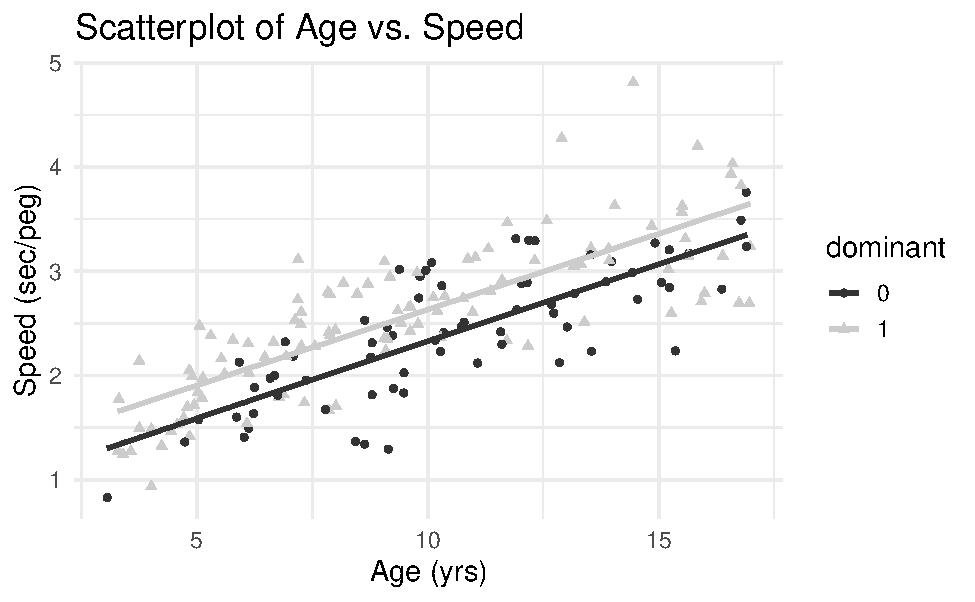
\includegraphics[width=0.7\linewidth]{10-regression_files/figure-latex/unnamed-chunk-6-1} \end{center}

\hypertarget{additional-notes}{%
\section{Additional notes}\label{additional-notes}}

Use this space to summarize your thoughts and take additional notes on today's activity.

\end{document}
